%\VignetteIndexEntry{EBSeq Vignette}

\documentclass{article}
\usepackage{fullpage}
\usepackage{graphicx, graphics, epsfig,setspace,amsmath, amsthm}
\usepackage{hyperref}
\usepackage{natbib}
%\usepackage{listings}
\usepackage{moreverb}
\usepackage{Sweave}
\begin{document}
\Sconcordance{concordance:EBSeq_Vignette.tex:EBSeq_Vignette.Rnw:%
1 9 1 1 0 164 1 1 2 4 0 1 2 22 1 1 2 1 0 1 1 9 0 1 2 5 1 1 2 4 0 1 2 23 %
1 1 5 11 0 2 2 1 0 1 1 5 0 1 1 11 0 1 1 7 0 1 2 42 1 1 2 1 0 1 1 11 0 2 %
1 8 0 2 1 3 0 1 2 4 1 1 2 4 0 1 2 18 1 1 2 1 0 2 1 7 0 1 2 9 1 1 3 8 0 %
2 1 5 0 1 1 11 0 1 1 7 0 1 2 20 1 1 2 1 0 1 1 9 0 1 2 3 1 1 2 4 0 1 2 2 %
1 1 2 1 0 1 2 8 0 1 2 1 1 1 2 1 0 1 1 11 0 1 2 5 1 1 2 1 0 1 1 5 0 1 1 %
15 0 1 1 8 0 1 1 11 0 1 2 16 1 1 2 1 0 7 1 3 0 1 2 4 1 1 5 11 0 1 2 2 1 %
1 2 1 0 1 1 18 0 1 2 2 1 1 2 1 0 1 1 5 0 1 1 37 0 1 1 8 0 1 1 18 0 1 2 %
14 1 1 2 1 0 1 1 1 2 1 0 1 1 3 0 1 3 1 0 1 1 5 0 1 1 11 0 1 1 7 0 1 2 7 %
1 1 2 1 0 1 1 9 0 1 1 4 0 1 2 17 1 1 2 6 0 1 1 5 0 1 1 6 0 1 2 16 1 1 2 %
1 0 1 1 4 0 1 2 13 1 1 2 1 0 1 1 4 0 1 2 18 1 1 2 1 0 4 1 3 0 1 3 6 0 2 %
1 7 0 1 2 28 1 1 2 4 0 1 2 10 1 1 2 1 0 1 2 7 0 1 1 3 0 1 3 14 0 1 2 2 %
1 1 2 1 0 1 1 10 0 1 2 7 1 1 2 6 0 1 1 5 0 1 1 6 0 1 2 16 1 1 2 1 0 1 1 %
1 5 9 0 1 3 10 1 1 2 1 0 3 1 1 2 1 0 1 2 1 0 1 2 1 0 1 2 5 0 1 2 10 1 1 %
2 1 0 1 1 4 0 1 2 9 1 1 2 1 0 1 1 4 0 1 2 11 1 1 2 1 0 2 1 1 3 5 0 1 2 %
1 1 1 2 1 0 1 1 5 0 1 1 15 0 1 1 8 0 1 1 11 0 1 2 5 1 1 2 1 0 1 1 10 0 %
1 1 4 0 1 2 8 1 1 2 1 0 1 1 27 0 1 2 6 1 1 2 1 0 1 1 4 0 1 2 5 1 1 2 1 %
0 1 1 4 0 1 2 10 1 1 2 1 0 7 1 1 2 1 0 1 1 3 0 1 3 6 0 1 1 37 0 1 1 8 0 %
1 1 17 0 1 1 3 0 1 2 3 1 1 2 1 0 1 1 18 0 1 2 2 1 1 2 5 0 1 2 14 1 1 2 %
1 0 1 1 5 0 1 3 7 1 1 2 1 0 1 1 4 0 1 2 29 1 1 2 1 0 2 1 1 3 10 0 2 1 3 %
0 1 2 7 1 1 2 1 0 7 1 1 3 10 0 2 1 3 0 1 2 6 1 1 2 1 0 2 1 1 3 2 0 1 3 %
8 0 2 1 3 0 1 2 9 1 1 2 1 0 8 1 1 7 12 0 2 1 3 0 1 2 141 1}

\title{EBSeq: An R package for differential expression analysis using RNA-seq data}
\author{Ning Leng, John Dawson, Xiuyu Ma, Michael A. Newton, and Christina Kendziorski}
\maketitle
\tableofcontents
\setcounter{tocdepth}{2}

\section{Introduction}
EBSeq may be used to identify differentially expressed (DE)
genes and isoforms in an RNA-Seq experiment. As detailed in
Leng {\it et al.}, 2013 \cite{Leng13}, 
EBSeq is an empirical Bayesian approach that models a number of features
observed in RNA-seq data. Importantly, for isoform level inference,
EBSeq directly accommodates isoform expression estimation uncertainty by
modeling the differential variability observed in distinct groups of isoforms.
Consider Figure 1, where we have plotted variance against mean
for all isoforms using RNA-Seq expression data from Leng {\it et al.}, 2013 \cite{Leng13}.
Also shown is the fit within three sub-groups of isoforms defined
by the number of constituent isoforms of the parent gene.
An isoform of gene $g$ is assigned to the $I_g=k$ group, where $k=1,2,3$,
if the total number of isoforms from gene $g$ is $k$ (the $I_g=3$ group contains
all isoforms from genes having 3 or more isoforms).
As shown in Figure 1, there is decreased variability in the $I_g=1$ group,
but increased variability in the others, due to the relative increase in
uncertainty inherent in estimating isoform expression when multiple isoforms of a given gene are
present.  If this structure is not accommodated, there is reduced power for
identifying isoforms in the $I_g=1$ group (since the true variances in that group are
lower, on average, than that derived from the full collection of isoforms) as well as increased
false discoveries in the $I_g=2$ and $I_g=3$ groups (since the true variances are higher, on average,
than those derived from the full collection). EBSeq directly models differential variability
as a function of $I_g$ providing a powerful approach for isoform level inference. As shown in Leng {\it et al.}, 2013
\cite{Leng13}, the model is also useful for identifying DE genes.
One bottleneck of the model is that the number of DE patterns is growing factorially with the number of conditions($K$) for comparison (Bell number), which makes the computation infeasible for big $K$. In EBSeq.2, we provide a pruning scheme by removing those unlikely patterns and greatly reducing the size of patterns. We utilize a one-step EM and rewrite the code in C++ for further efficiency.
We will briefly detail the model in Section \ref{sec:model} and then describe
the flow of analysis in Section \ref{sec:quickstart} for both isoform and gene-level inference.


\begin{figure}[t]
\centering
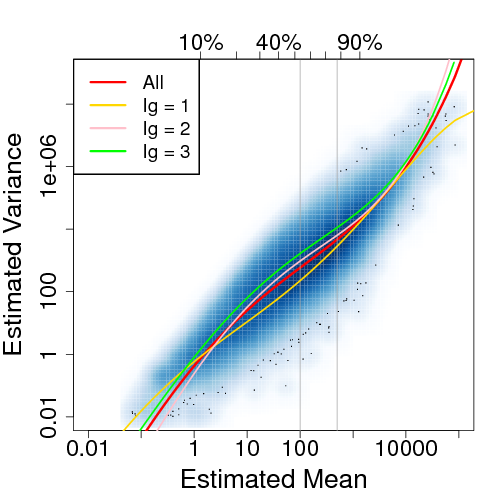
\includegraphics[width=0.6\textwidth]{PlotExample.png}
\label{fig:GouldNg}
\caption{Empirical variance vs. mean for
each isoform profiled in the ESCs vs iPSCs experiment detailed in
the Case Study section of Leng {\it et al.}, 2013 \cite{Leng13}.
A spline fit to all isoforms is shown in red with splines fit within the $I_g=1$, $I_g=2$, and $I_g=3$ isoform groups
shown in yellow, pink, and green, respectively.}
\end{figure}


\section{Citing this software}
\label{sec:cite}
Please cite the following article when reporting results from the software.

\noindent Leng, N., J.A. Dawson, J.A. Thomson, V. Ruotti, A.I. Rissman, 
B.M.G. Smits, J.D. Haag, M.N. Gould, R.M. Stewart, and C. Kendziorski. 
EBSeq: An empirical Bayes hierarchical model for inference in RNA-seq
experiments, {\it Bioinformatics}, 2013.

\section{The Model}
\label{sec:model}
\subsection{Two conditions}
\label{sec:twocondmodel}
We let $X_{g_i}^{C1} = X_{g_i,1} ,X_{g_i,2}, ...,X_{g_i,S_1}$ denote data from condition 1
and $ X_{g_i}^{C2} = X_{g_i,(S_1+1)},X_{g_i,(S_1+2)},...,X_{g_i,S}$ data from condition 2.
We assume that counts within condition $C$ are distributed as Negative Binomial: 
$X_{g_i,s}^C|r_{g_i,s}, q_{g_i}^C \sim NB(r_{g_i,s}, q_{g_i}^C)$ where
\begin{equation}
P(X_{g_i,s}|r_{g_i,s},q_{g_i}^C) = {X_{g_i,s}+r_{g_i,s}-1\choose X_{g_i,s}}(1-q_{g_i}^C)^{X_{g_i,s}}(q_{g_i}^C)^{r_{g_i,s}}\label{eq:01}
\end{equation}

\noindent and $\mu_{g_i,s}^C=r_{g_i,s} (1-q_{g_i}^C)/q_{g_i}^C$;
$(\sigma_{g_i,s}^C)^2=r_{g_i,s} (1-q_{g_i}^C)/(q_{g_i}^C)^2.$

\medskip

We assume a prior distribution on $q_{g_i}^C$: $q_{g_i}^C|\alpha, \beta^{I_g} \sim Beta(\alpha, \beta^{I_g})$.
The hyperparameter $\alpha$ is shared by all the isoforms and $\beta^{I_g}$ is $I_g$ specific (note this is an index, not a power).
We further assume that $r_{g_i,s}=r_{g_i,0} l_s$, where $r_{g_i,0}$ is an isoform specific 
parameter common across conditions and $r_{g_i,s}$ depends on it through the sample-specific normalization factor $l_s$.
Of interest in this two group comparison is distinguishing between two cases, or what we will refer to subsequently as
two patterns of expression, namely equivalent expression (EE) and differential expression (DE):
\begin{center}
$H_0$ (EE) : $q_{g_i}^{C1}=q_{g_i}^{C2}$  vs  $H_1$ (DE) : $q_{g_i}^{C1} \neq q_{g_i}^{C2}$.
\end{center}
Under the null hypothesis (EE), the data $X_{g_i}^{C1,C2} = X_{g_i}^{C1}, X_{g_i}^{C2}$ arises 
from the prior predictive distribution $f_0^{I_g}(X_{g_i}^{C1,C2})$:
%\tiny
\begin{equation}
f_0^{I_g}(X_{g_i}^{C1,C2})=\Bigg[\prod_{s=1}^S {X_{g_i,s}+r_{g_i,s}-1\choose X_{g_i,s}}\Bigg]
\frac{Beta(\alpha+\sum_{s=1}^S r_{g_i,s}, \beta^{I_g}+\sum_{s=1}^SX_{g_i,s} )}{Beta(\alpha, \beta^{I_g})}\label{eq:05}
\end{equation}
%\normalsize

Alternatively (in a DE scenario), $X_{g_i}^{C1,C2}$ follows the prior predictive distribution $f_1^{I_g}(X_{g_i}^{C1,C2})$:
\begin{equation}
f_1^{I_g}(X_{g_i}^{C1,C2})=f_0^{I_g}(X_{g_i}^{C1})f_0^{I_g}(X_{g_i}^{C2}) \label{eq:06}
\end{equation}

Let the latent variable $Z_{g_i}$ be defined so that $Z_{g_i} = 1$ indicates that 
isoform $g_i$ is DE and $Z_{g_i} =  0$ indicates isoform $g_i$ is EE, and
$Z_{g_i} \sim Bernoulli(p)$.
Then, the marginal distribution of $X_{g_i}^{C1,C2}$ and $Z_{g_i}$ is:
\begin{equation}
(1-p)f_0^{I_g}(X_{g_i}^{C1,C2}) + pf_1^{I_g}(X_{g_i}^{C1,C2})\label{eq:07}
\end{equation}

\noindent The posterior probability of being DE at isoform $g_i$ is obtained by Bayes' rule:
\begin{equation}
\frac{pf_1^{I_g}(X_{g_i}^{C1,C2})}{(1-p)f_0^{I_g}(X_{g_i}^{C1,C2}) + pf_1^{I_g}(X_{g_i}^{C1,C2})}\label{eq:08}
\end{equation}

%\newpage
\subsection{More than two conditions}
\label{sec:multicondmodel}
EBSeq naturally accommodates multiple condition comparisons.
For example, in a study with 3 conditions, there are K=5 possible expression patterns (P1,...,P5), or ways in which
latent levels of expression may vary across conditions:
\begin{align}
\textrm {P1:}& \hspace{0.05in} q_{g_i}^{C1} = q_{g_i}^{C2}=q_{g_i}^{C3} \nonumber \\
\textrm {P2:}& \hspace{0.05in} q_{g_i}^{C1} = q_{g_i}^{C2} \neq q_{g_i}^{C3} \nonumber \\
\textrm {P3:}& \hspace{0.05in} q_{g_i}^{C1} = q_{g_i}^{C3} \neq q_{g_i}^{C2} \nonumber \\
\textrm {P4:}& \hspace{0.05in} q_{g_i}^{C1} \neq q_{g_i}^{C2} = q_{g_i}^{C3} \nonumber \\
\textrm {P5:}& \hspace{0.05in} q_{g_i}^{C1} \neq q_{g_i}^{C2} \neq
q_{g_i}^{C3} \textrm{ and } q_{g_i}^{C1} \neq q_{g_i}^{C3} \nonumber
\end{align}

\noindent The prior predictive distributions for these are given, respectively, by:

\begin{align}
g_1^{I_g}(X_{g_i}^{C1,C2,C3}) &= f_0^{I_g}(X_{g_i}^{C1,C2,C3}) \nonumber \\
g_2^{I_g}(X_{g_i}^{C1,C2,C3}) &= f_0^{I_g}(X_{g_i}^{C1,C2})f_0^{I_g}(X_{g_i}^{C3}) \nonumber \\
g_3^{I_g}(X_{g_i}^{C1,C2,C3}) &= f_0^{I_g}(X_{g_i}^{C1,C3})f_0^{I_g}(X_{g_i}^{C2}) \nonumber \\
g_4^{I_g}(X_{g_i}^{C1,C2,C3}) &= f_0^{I_g}(X_{g_i}^{C1})f_0^{I_g}(X_{g_i}^{C2,C3}) \nonumber \\
g_5^{I_g}(X_{g_i}^{C1,C2,C3}) &= f_0^{I_g}(X_{g_i}^{C1})f_0^{I_g}(X_{g_i}^{C2})f_0^{I_g}(X_{g_i}^{C3}) \nonumber
\end{align}

\noindent where $f_0^{I_g}$ is the same as in equation \ref{eq:05}. Then the marginal distribution in 
equation \ref{eq:07} becomes:

\begin{equation}
\sum_{k=1}^5 p_k g_k^{I_g}(X_{g_i}^{C1,C2,C3}) \label{eq:11}
\end{equation}
\noindent where $\sum_{k=1}^5 p_k = 1$. Thus, the posterior probability of
isoform $g_i$ coming from pattern $K$ is readily obtained by:

\begin{equation}
\frac{p_K g_K^{I_g}(X_{g_i}^{C1,C2,C3})}{\sum_{k=1}^5 p_k g_k^{I_g}(X_{g_i}^{C1,C2,C3})} \label{eq:12}
\end{equation}

\subsection{Getting a false discovery rate (FDR) controlled list of genes or isoforms}
\label{sec:fdrlist}
To obtain a list of DE genes with false discovery rate (FDR) controlled
at $\alpha$ in an experiment comparing two biological conditions, the genes
with posterior probability of being DE (PPDE) greater than 1 - $\alpha$ should be used.
For example, the genes with PPDE>=0.95 make up the list of DE genes with target
FDR controlled at 5\%.  With more than two biological conditions, there are multiple
DE patterns (see Section \ref{sec:multicondmodel}). To obtain a list of genes in a specific DE pattern with target
FDR $\alpha$, a user should
take the genes with posterior probability of being in that pattern greater
than 1 - $\alpha$. Isoform-based lists are obtained in the same way.
\newpage
\section{Quick Start}
\label{sec:quickstart}
Before analysis can proceed, the EBSeq package must be loaded into the working space:
\begin{Schunk}
\begin{Sinput}
> library(EBSeq)
\end{Sinput}
\end{Schunk}
\subsection{Gene level DE analysis (two conditions)}
\label{sec:startgenede}
\subsubsection{Required input}
\label{sec:startgenedeinput}
\begin{flushleft}
{\bf Data}:  The object \verb+Data+ should be a $G-by-S$ matrix containing the expression values for each gene and each sample,
where $G$ is the number of genes and $S$ is the number of samples. These
values should exhibit raw counts, without normalization
across samples. Counts of this nature may be obtained from RSEM \cite{Li11b},
Cufflinks \cite{Trapnell12}, or a similar approach.

\vspace{5 mm}

{\bf Conditions}:  The object \verb+Conditions+ should be a Factor vector of length $S$ that indicates to which condition each sample belongs.
For example, if there are two conditions and three samples in each,
$S=6$ and \verb+Conditions+ may be given by 

\verb+as.factor(c("C1","C1","C1","C2","C2","C2"))+

\end{flushleft} 
\noindent The object \verb+GeneMat+ is a simulated data matrix containing 
1,000 rows of genes and 10 columns of samples. The genes are named 
\verb+Gene_1, Gene_2 ...+
\begin{Schunk}
\begin{Sinput}
> data(GeneMat)
> str(GeneMat)
\end{Sinput}
\begin{Soutput}
 num [1:1000, 1:10] 1879 24 3291 97 485 ...
 - attr(*, "dimnames")=List of 2
  ..$ : chr [1:1000] "Gene_1" "Gene_2" "Gene_3" "Gene_4" ...
  ..$ : NULL
\end{Soutput}
\end{Schunk}

\subsubsection{Library size factor}
\label{sec:startgenedesize}
As detailed in Section \ref{sec:model}, EBSeq requires the library size factor $l_s$ for each sample $s$.
Here, $l_s$ may be obtained via the function \verb+MedianNorm+, which reproduces the median normalization approach
in DESeq \citep{Anders10}.
\begin{Schunk}
\begin{Sinput}
> Sizes=MedianNorm(GeneMat)
\end{Sinput}
\end{Schunk}

\noindent If quantile normalization is preferred, $l_s$ may be obtained via the function \verb+QuantileNorm+. 
(e.g. \verb+QuantileNorm(GeneMat,.75)+ for Upper-Quantile Normalization in \cite{Bullard10})

\subsubsection{Running EBSeq on gene expression estimates}
\label{sec:startgenederun}
The function \verb+EBTest+ is used to detect DE genes. 
For gene-level data, we don't need to specify the parameter 
\verb+NgVector+ since there are no differences in $I_g$ structure among the different genes.
Here, we simulated the first five samples to be in condition 1 and the other five in condition 2, so define: 

\verb+Conditions=as.factor(rep(c("C1","C2"),each=5))+

\noindent \verb+sizeFactors+ is used to define the library size factor of each sample. 
It could be obtained by summing up the total number of reads within each sample, 
Median Normalization \citep{Anders10},
scaling normalization \citep{Robinson10}, Upper-Quantile Normalization \cite{Bullard10}, 
or some other such approach.
These in hand, we run the EM algorithm, setting the number 
of iterations to five via \verb+maxround=5+ for demonstration purposes. 
However, we note that in practice, 
additional iterations are usually required. Convergence should always be 
checked (see Section \ref{sec:detailedgenedeconverge} for details).
Please note this may take several minutes:
\begin{Schunk}
\begin{Sinput}
> #EBOut=EBTest(Data=GeneMat, 
> #Conditions=as.factor(rep(c("C1","C2"),each=5)),sizeFactors=Sizes, maxround=5)
> EBOut = EBTest(Data=GeneMat, Conditions=as.factor(rep(c("C1","C2"),each=5)),
+        sizeFactors = Sizes)
\end{Sinput}
\begin{Soutput}
Initial number of DE patterns = 2
Final number of DE patterns = 2
\end{Soutput}
\end{Schunk}
\noindent The list of DE genes and the posterior probabilities of being DE are obtained as follows
\begin{Schunk}
\begin{Sinput}
> EBDERes=GetDEResults(EBOut, FDR=0.05)
> str(EBDERes$DEfound)
\end{Sinput}
\begin{Soutput}
 chr [1:94] "Gene_1" "Gene_2" "Gene_3" "Gene_4" "Gene_5" "Gene_6" "Gene_7" ...
\end{Soutput}
\begin{Sinput}
> head(EBDERes$PPMat)
\end{Sinput}
\begin{Soutput}
                PPEE PPDE
Gene_1  0.000000e+00    1
Gene_2  6.831008e-47    1
Gene_3 1.070213e-218    1
Gene_4  2.085332e-33    1
Gene_5 1.907801e-229    1
Gene_6  1.170782e-09    1
\end{Soutput}
\begin{Sinput}
> str(EBDERes$Status)
\end{Sinput}
\begin{Soutput}
 Named chr [1:1000] "DE" "DE" "DE" "DE" "DE" "DE" "DE" "DE" "DE" "DE" "DE" ...
 - attr(*, "names")= chr [1:1000] "Gene_1" "Gene_2" "Gene_3" "Gene_4" ...
\end{Soutput}
\end{Schunk}
\noindent \verb+EBDERes$DEfound+ is a list of genes identified with 5\% FDR. EBSeq found
95 genes. The matrix \verb+EBDERes$PPMat+ contains two columns \verb+PPEE+ and \verb+PPDE+, 
corresponding to the posterior probabilities of being EE or DE for each gene. 
\verb+EBDERes$Status+ contains each gene's status called by EBSeq. 

\noindent Note the \verb+GetDEResults()+ was incorporated in EBSeq since version 1.7.1. 
By using the default settings, the number of genes identified in any given analysis may 
differ slightly from the previous version. The updated algorithm is more robust to outliers
and transcripts with low variance. To obtain results that are comparable
to results from earlier versions of EBSeq ($\le$ 1.7.0), a user may set
\verb+Method="classic"+ in \verb+GetDEResults()+ function, or use the \verb+GetPPMat()+ function.


\subsection{Isoform level DE analysis (two conditions)}
\label{sec:startisode}
\subsubsection{Required inputs}
\label{sec:startisodeinput}

\begin{flushleft}
{\bf Data}:   The object \verb+Data+ should be a $I-by-S$ matrix containing the expression values for each isoform and each sample,
where $I$ is the number of isoforms and $S$ is the number of sample. As in the gene-level analysis, these values should exhibit raw data, without normalization
across samples.

\vspace{5 mm}

{\bf Conditions}:  The object \verb+Conditions+ should be a vector with length $S$ to indicate the condition of each sample.

\vspace{5 mm}

{\bf IsoformNames}:   The object \verb+IsoformNames+ should be a vector with length $I$ to indicate the isoform names.

\vspace{5 mm}

{\bf IsosGeneNames}:  The object \verb+IsosGeneNames+ should be a vector with length $I$ to indicate the gene name of each isoform. 
(in the same order as \verb+IsoformNames+.)
\end{flushleft}

\noindent \verb+IsoList+ contains 1,200 simulated isoforms. 
In which \verb+IsoList$IsoMat+ is a data matrix containing
1,200 rows of isoforms and 10 columns of samples; 
\verb+IsoList$IsoNames+ contains the isoform names; 
\verb+IsoList$IsosGeneNames+ contains the names of the genes the isoforms belong to.

\begin{Schunk}
\begin{Sinput}
> data(IsoList)
> str(IsoList)
\end{Sinput}
\begin{Soutput}
List of 3
 $ IsoMat       : num [1:1200, 1:10] 176 789 1300 474 1061 ...
  ..- attr(*, "dimnames")=List of 2
  .. ..$ : chr [1:1200] "Iso_1_1" "Iso_1_2" "Iso_1_3" "Iso_1_4" ...
  .. ..$ : NULL
 $ IsoNames     : chr [1:1200] "Iso_1_1" "Iso_1_2" "Iso_1_3" "Iso_1_4" ...
 $ IsosGeneNames: chr [1:1200] "Gene_1" "Gene_2" "Gene_3" "Gene_4" ...
\end{Soutput}
\begin{Sinput}
> IsoMat=IsoList$IsoMat
> str(IsoMat)
\end{Sinput}
\begin{Soutput}
 num [1:1200, 1:10] 176 789 1300 474 1061 ...
 - attr(*, "dimnames")=List of 2
  ..$ : chr [1:1200] "Iso_1_1" "Iso_1_2" "Iso_1_3" "Iso_1_4" ...
  ..$ : NULL
\end{Soutput}
\begin{Sinput}
> IsoNames=IsoList$IsoNames
> IsosGeneNames=IsoList$IsosGeneNames
\end{Sinput}
\end{Schunk}

\subsubsection{Library size factor}
\label{sec:startisodesize}
Similar to the gene-level analysis presented above, we may obtain the isoform-level 
library size factors via \verb+MedianNorm+:
\begin{Schunk}
\begin{Sinput}
> IsoSizes=MedianNorm(IsoMat)
\end{Sinput}
\end{Schunk}

\subsubsection{The $I_g$ vector}
\label{sec:startisodeNg}

While working on isoform level data, EBSeq fits different prior 
parameters for different uncertainty groups (defined as $I_g$ groups).
The default setting to define the uncertainty groups consists of using 
the number of isoforms the host gene contains ($N_g$) for each isoform. 
The default settings will provide three uncertainty groups: 

$I_g=1$ group: Isoforms with $N_g=1$;

$I_g=2$ group: Isoforms with $N_g=2$;

$I_g=3$ group: Isoforms with $N_g \geq 3$.

The $N_g$ and $I_g$ group assignment can be obtained using the function \verb+GetNg+. 
The required inputs of \verb+GetNg+ are the isoform names (\verb+IsoformNames+) and 
their corresponding gene names (\verb+IsosGeneNames+).
\begin{Schunk}
\begin{Sinput}
> NgList=GetNg(IsoNames, IsosGeneNames)
> IsoNgTrun=NgList$IsoformNgTrun
> IsoNgTrun[c(1:3,201:203,601:603)]
\end{Sinput}
\begin{Soutput}
Iso_1_1 Iso_1_2 Iso_1_3 Iso_2_1 Iso_2_2 Iso_2_3 Iso_3_1 Iso_3_2 Iso_3_3 
      1       1       1       2       2       2       3       3       3 
\end{Soutput}
\end{Schunk}
More details could be found in Section \ref{sec:detailedisode}.

\subsubsection{Running EBSeq on isoform expression estimates}
\label{sec:startisoderun}
The \verb+EBTest+ function is also used to run EBSeq for two condition comparisons 
on isoform-level data. 
Below we use 5 iterations to demonstrate.  However, as
in the gene level analysis, we advise that additional iterations will likely be 
required in practice (see Section \ref{sec:detailedisodeconverge} for details). 

\begin{Schunk}
\begin{Sinput}
> IsoEBOut = EBTest(Data=IsoMat, NgVector=IsoNgTrun, 
+ Conditions=as.factor(rep(c("C1","C2"),each=5)),sizeFactors=IsoSizes)
\end{Sinput}
\begin{Soutput}
Initial number of DE patterns = 2
Final number of DE patterns = 2
\end{Soutput}
\begin{Sinput}
> IsoEBDERes=GetDEResults(IsoEBOut, FDR=0.05)
> str(IsoEBDERes$DEfound)
\end{Sinput}
\begin{Soutput}
 chr [1:104] "Iso_1_1" "Iso_1_2" "Iso_1_3" "Iso_1_4" "Iso_1_5" "Iso_1_6" ...
\end{Soutput}
\begin{Sinput}
> head(IsoEBDERes$PPMat)
\end{Sinput}
\begin{Soutput}
                 PPEE PPDE
Iso_1_1  1.179612e-18    1
Iso_1_2  2.440508e-83    1
Iso_1_3  0.000000e+00    1
Iso_1_4 5.585848e-206    1
Iso_1_5  3.898363e-71    1
Iso_1_6  8.466569e-55    1
\end{Soutput}
\begin{Sinput}
> str(IsoEBDERes$Status)
\end{Sinput}
\begin{Soutput}
 Named chr [1:1200] "DE" "DE" "DE" "DE" "DE" "DE" "DE" "DE" "DE" "DE" "DE" ...
 - attr(*, "names")= chr [1:1200] "Iso_1_1" "Iso_1_2" "Iso_1_3" "Iso_1_4" ...
\end{Soutput}
\end{Schunk}
\noindent We see that EBSeq found 104 DE isoforms at the target FDR of 0.05. 

\noindent Note the \verb+GetDEResults()+ was incorporated in EBSeq since version 1.7.1.
By using the default settings, the number of transcripts identified in any given analysis may 
differ slightly from the previous version. The updated algorithm is more robust to outliers
and transcripts with low variance. To obtain results that are comparable
to results from earlier versions of EBSeq ($\le$ 1.7.0), a user may set
\verb+Method="classic"+ in \verb+GetDEResults()+ function, or use the \verb+GetPPMat()+ function.






\subsection{Gene level DE analysis (more than two conditions)}
\label{sec:startmulticond}
\noindent The object \verb+MultiGeneMat+ is a matrix containing 
500 simulated genes with 6 samples: 
the first two samples are from condition 1; the second and the third sample are 
from condition 2; the last two samples are from condition 3.

\begin{Schunk}
\begin{Sinput}
> data(MultiGeneMat)
> str(MultiGeneMat)
\end{Sinput}
\begin{Soutput}
 num [1:500, 1:6] 411 268 768 1853 878 ...
 - attr(*, "dimnames")=List of 2
  ..$ : chr [1:500] "Gene_1" "Gene_3" "Gene_5" "Gene_7" ...
  ..$ : NULL
\end{Soutput}
\end{Schunk}
In analysis where the data are spread over more than two conditions,
the set of possible patterns for each gene is more complicated
than simply EE and DE. As noted in Section \ref{sec:model}, when we have 3 conditions, there are 5 expression
patterns to consider. In the simulated data, we have 6 samples, 2 in each of 3 conditions.
\begin{Schunk}
\begin{Sinput}
> Conditions=c("C1","C1","C2","C2","C3","C3")
\end{Sinput}
\end{Schunk}

\verb+MedianNorm+ or one of its competitors should be used to determine the normalization factors.
Once this is done, the formal test is performed by \verb+EBMultiTest+. 
\begin{Schunk}
\begin{Sinput}
> MultiSize=MedianNorm(MultiGeneMat)
> MultiOut=EBMultiTest(MultiGeneMat,Conditions=Conditions,
+  sizeFactors=MultiSize, uc = 2)
\end{Sinput}
\begin{Soutput}
Initial number of DE patterns = 5
Final number of DE patterns = 5
\end{Soutput}
\end{Schunk}
The function \verb+GetPatterns+ allows the user to get selected patterns. For example:

\begin{Schunk}
\begin{Sinput}
> PosParti=GetPatterns(MultiOut)
> PosParti
\end{Sinput}
\begin{Soutput}
         C1 C2 C3
Pattern1  1  2  3
Pattern2  1  1  2
Pattern3  1  2  2
Pattern4  1  1  1
Pattern5  1  2  1
\end{Soutput}
\end{Schunk}

\noindent where the first row means all three conditions have distinct latent mean expression level; 
the second row means C1 and C2 have the same latent mean expression level but that of C3 is different; 
and the last row corresponds to the case where C1 and C3 have the same latent mean expression level but that of C2 is different.
\noindent The posterior probability of being in each pattern for every gene is obtained by using the 
function \verb+GetMultiPP+:
\begin{Schunk}
\begin{Sinput}
> MultiPP=GetMultiPP(MultiOut)
> names(MultiPP)
\end{Sinput}
\begin{Soutput}
[1] "PP"       "MAP"      "Patterns"
\end{Soutput}
\begin{Sinput}
> MultiPP$PP[1:10,]
\end{Sinput}
\begin{Soutput}
           pattern1  pattern2      pattern3      pattern4      pattern5
Gene_1  0.342709563 0.6572904  6.870408e-72  3.015440e-93  2.864790e-55
Gene_3  0.006595105 0.9934049 5.340316e-109 3.433672e-163 2.922145e-116
Gene_5  0.042482476 0.9575175  5.309949e-20  7.837887e-26  1.140460e-18
Gene_7  0.157609361 0.8423906  0.000000e+00  0.000000e+00 2.905691e-294
Gene_9  0.040619174 0.9593808  2.441999e-15  9.088562e-16  9.343836e-16
Gene_11 0.053841782 0.9461582  2.607784e-12  2.955394e-11  4.570651e-11
Gene_13 0.106486219 0.8935129  9.194008e-10  6.798796e-08  7.735994e-07
Gene_15 0.027054430 0.9729456  1.079379e-40  5.379139e-47  2.410435e-44
Gene_17 0.181376143 0.8186239 4.590012e-133 7.310837e-184 9.831129e-113
Gene_19 0.048700449 0.9512996  1.080862e-24  2.792245e-37  6.753301e-28
\end{Soutput}
\begin{Sinput}
> MultiPP$MAP[1:10]
\end{Sinput}
\begin{Soutput}
    Gene_1     Gene_3     Gene_5     Gene_7     Gene_9    Gene_11    Gene_13 
"pattern2" "pattern2" "pattern2" "pattern2" "pattern2" "pattern2" "pattern2" 
   Gene_15    Gene_17    Gene_19 
"pattern2" "pattern2" "pattern2" 
\end{Soutput}
\begin{Sinput}
> MultiPP$Patterns
\end{Sinput}
\begin{Soutput}
         C1 C2 C3
Pattern1  1  2  3
Pattern2  1  1  2
Pattern3  1  2  2
Pattern4  1  1  1
Pattern5  1  2  1
\end{Soutput}
\end{Schunk}
\noindent where \verb+MultiPP$PP+ provides the posterior probability of being in each pattern for every gene. 
\verb+MultiPP$MAP+ provides the most likely pattern of each gene based on the posterior 
probabilities. \verb+MultiPP$Patterns+ provides the details of the patterns. 



\subsection{Isoform level DE analysis (more than two conditions)}
\label{sec:startisomulticond}
\noindent Similar to \verb+IsoList+,
the object \verb+IsoMultiList+ is an object containing the isoform expression estimates matrix, the isoform 
names, and the gene names of the isoforms' host genes. 
\verb+IsoMultiList$IsoMultiMat+ contains 300 simulated isoforms with 8 samples. 
The first two samples are from condition 1; the second and the third sample are 
from condition 2; the fifth and sixth sample are from condition 3; 
the last two samples are from condition 4.
Similar to Section \ref{sec:startisode},  the function \verb+MedianNorm+ and \verb+GetNg+ could be used for normalization 
and calculating the $N_g$'s. 
\begin{Schunk}
\begin{Sinput}
> data(IsoMultiList)
> IsoMultiMat=IsoMultiList[[1]]
> IsoNames.Multi=IsoMultiList$IsoNames
> IsosGeneNames.Multi=IsoMultiList$IsosGeneNames
> IsoMultiSize=MedianNorm(IsoMultiMat)
> NgList.Multi=GetNg(IsoNames.Multi, IsosGeneNames.Multi)
> IsoNgTrun.Multi=NgList.Multi$IsoformNgTrun
> Conditions=c("C1","C1","C2","C2","C3","C3","C4","C4")
\end{Sinput}
\end{Schunk}



\noindent
\verb+EBMultiTest+ could be used to perform the test:
\begin{Schunk}
\begin{Sinput}
> IsoMultiOut=EBMultiTest(IsoMultiMat,
+ NgVector=IsoNgTrun.Multi,Conditions=Conditions,
+ sizeFactors=IsoMultiSize, 
+ uc = 2,nequal = 10)
\end{Sinput}
\begin{Soutput}
Initial number of DE patterns = 12
Final number of DE patterns = 12
\end{Soutput}
\end{Schunk}

The function \verb+GetPatterns+ allows the user to get selected patterns. For example:

\begin{Schunk}
\begin{Sinput}
> PosParti.4Cond=GetPatterns(IsoMultiOut)
> PosParti.4Cond
\end{Sinput}
\begin{Soutput}
          C1 C2 C3 C4
Pattern1   1  1  1  2
Pattern2   1  1  2  3
Pattern3   1  2  2  3
Pattern4   1  2  1  3
Pattern5   1  2  3  4
Pattern6   1  1  1  1
Pattern7   1  2  1  2
Pattern8   1  1  2  1
Pattern9   1  2  1  1
Pattern10  1  1  2  2
Pattern11  1  2  2  2
Pattern12  1  2  3  2
\end{Soutput}
\end{Schunk}

\noindent The posterior probability of being in each pattern for every gene is obtained by using the 
function \verb+GetMultiPP+:
\begin{Schunk}
\begin{Sinput}
> IsoMultiPP=GetMultiPP(IsoMultiOut)
> names(MultiPP)
\end{Sinput}
\begin{Soutput}
[1] "PP"       "MAP"      "Patterns"
\end{Soutput}
\begin{Sinput}
> IsoMultiPP$PP[1:10,]
\end{Sinput}
\begin{Soutput}
             pattern1     pattern2     pattern3     pattern4     pattern5
Iso_1_1  9.944829e-01 2.487951e-03 1.268388e-03 1.758950e-03 1.771681e-06
Iso_1_2  9.912427e-01 2.969262e-03 3.149008e-03 2.634129e-03 4.875175e-06
Iso_1_3  9.511978e-01 3.810283e-02 8.491698e-03 2.162905e-03 4.476499e-05
Iso_1_4  9.894764e-01 5.116263e-03 2.454048e-03 2.946992e-03 6.317775e-06
Iso_1_5  9.991552e-01 7.293563e-05 1.735210e-04 5.983095e-04 2.165350e-08
Iso_1_6  5.281437e-05 9.992943e-01 7.313762e-07 3.257042e-05 6.196223e-04
Iso_1_7  9.934368e-01 1.784738e-03 2.173345e-03 2.602521e-03 2.640945e-06
Iso_1_8  8.288801e-01 1.595626e-01 1.813693e-03 9.599158e-03 1.444232e-04
Iso_1_9  7.704437e-01 2.182868e-01 2.149635e-03 8.906145e-03 2.136948e-04
Iso_1_10 9.913102e-01 3.714386e-03 2.129945e-03 2.838316e-03 4.514167e-06
              pattern6      pattern7      pattern8      pattern9     pattern10
Iso_1_1   6.547737e-32  7.334070e-28  7.444297e-33  1.187580e-33  7.826127e-30
Iso_1_2   6.429034e-14  2.381428e-15  3.864389e-16  1.449241e-15  4.027626e-15
Iso_1_3   1.182199e-46  6.734763e-38  9.816011e-42  1.000115e-47  9.124439e-46
Iso_1_4   6.216584e-35  1.237632e-20  2.301442e-30  6.596860e-32  7.318319e-23
Iso_1_5   0.000000e+00  0.000000e+00  0.000000e+00  0.000000e+00  0.000000e+00
Iso_1_6  4.033350e-234 4.955181e-156 1.142613e-221 3.682627e-183 3.684941e-101
Iso_1_7  5.630249e-138 6.431489e-104 1.006944e-132 2.204727e-135 3.261238e-110
Iso_1_8  1.467526e-138  2.610835e-67 3.869222e-105 8.031404e-123  4.969433e-88
Iso_1_9   3.352994e-47  2.274798e-45  1.364332e-50  1.007720e-43  8.001378e-30
Iso_1_10  5.983367e-08  1.870470e-06  1.057221e-09  1.094014e-09  6.574554e-07
             pattern11     pattern12
Iso_1_1   4.409921e-34  4.382372e-30
Iso_1_2   1.304877e-17  2.614705e-17
Iso_1_3   8.498244e-50  8.269050e-39
Iso_1_4   5.692183e-33  1.574014e-22
Iso_1_5   0.000000e+00  0.000000e+00
Iso_1_6  2.865219e-189 5.592363e-154
Iso_1_7  2.057379e-128 3.871764e-106
Iso_1_8  5.645298e-120  2.330319e-68
Iso_1_9   4.875946e-46  3.238016e-46
Iso_1_10  1.013843e-09  1.764817e-08
\end{Soutput}
\begin{Sinput}
> IsoMultiPP$MAP[1:10]
\end{Sinput}
\begin{Soutput}
   Iso_1_1    Iso_1_2    Iso_1_3    Iso_1_4    Iso_1_5    Iso_1_6    Iso_1_7 
"pattern1" "pattern1" "pattern1" "pattern1" "pattern1" "pattern2" "pattern1" 
   Iso_1_8    Iso_1_9   Iso_1_10 
"pattern1" "pattern1" "pattern1" 
\end{Soutput}
\begin{Sinput}
> IsoMultiPP$Patterns
\end{Sinput}
\begin{Soutput}
          C1 C2 C3 C4
Pattern1   1  1  1  2
Pattern2   1  1  2  3
Pattern3   1  2  2  3
Pattern4   1  2  1  3
Pattern5   1  2  3  4
Pattern6   1  1  1  1
Pattern7   1  2  1  2
Pattern8   1  1  2  1
Pattern9   1  2  1  1
Pattern10  1  1  2  2
Pattern11  1  2  2  2
Pattern12  1  2  3  2
\end{Soutput}
\end{Schunk}
\noindent where \verb+MultiPP$PP+ provides the posterior probability of being in each pattern for every gene. 
\verb+MultiPP$MAP+ provides the most likely pattern of each gene based on the posterior 
probabilities. \verb+MultiPP$Patterns+ provides the details of the patterns. 



\newpage
\section{More detailed examples}
\label{sec:detailed}
\subsection{Gene level DE analysis (two conditions)}
\label{sec:detailedgenede}

\subsubsection{Running EBSeq on simulated gene expression estimates}
\label{sec:detailedgenederun}
EBSeq is applied as described in Section \ref{sec:startgenederun}.
\begin{Schunk}
\begin{Sinput}
> data(GeneMat)
> Sizes=MedianNorm(GeneMat)
> EBOut=EBTest(Data=GeneMat, 
+ Conditions=as.factor(rep(c("C1","C2"),each=5)),sizeFactors=Sizes)
> EBDERes=GetDEResults(EBOut, FDR=0.05)
\end{Sinput}
\end{Schunk}
\begin{Schunk}
\begin{Sinput}
> EBDERes=GetDEResults(EBOut, FDR=0.05)
> str(EBDERes$DEfound)
\end{Sinput}
\begin{Soutput}
 chr [1:94] "Gene_1" "Gene_2" "Gene_3" "Gene_4" "Gene_5" "Gene_6" "Gene_7" ...
\end{Soutput}
\begin{Sinput}
> head(EBDERes$PPMat)
\end{Sinput}
\begin{Soutput}
                PPEE PPDE
Gene_1  0.000000e+00    1
Gene_2  6.831008e-47    1
Gene_3 1.070213e-218    1
Gene_4  2.085332e-33    1
Gene_5 1.907801e-229    1
Gene_6  1.170782e-09    1
\end{Soutput}
\begin{Sinput}
> str(EBDERes$Status)
\end{Sinput}
\begin{Soutput}
 Named chr [1:1000] "DE" "DE" "DE" "DE" "DE" "DE" "DE" "DE" "DE" "DE" "DE" ...
 - attr(*, "names")= chr [1:1000] "Gene_1" "Gene_2" "Gene_3" "Gene_4" ...
\end{Soutput}
\end{Schunk}
\noindent EBSeq found 94 DE genes at a target FDR of 0.05.\\

\subsubsection{Calculating FC}
\label{sec:detailedgenedefc}
The function \verb+PostFC+ may be used to calculate the Fold Change (FC) 
of the raw data as well as the posterior FC of the normalized data.
\begin{figure}[h!]
\centering
\begin{Schunk}
\begin{Sinput}
> GeneFC=PostFC(EBOut)
> str(GeneFC)
\end{Sinput}
\begin{Soutput}
List of 3
 $ PostFC   : num [1:1000, 1] 0.237 0.241 4.127 4.237 3.909 ...
 $ RealFC   : Named num [1:1000] 0.237 0.239 4.128 4.28 3.918 ...
  ..- attr(*, "names")= chr [1:1000] "Gene_1" "Gene_2" "Gene_3" "Gene_4" ...
 $ Direction: chr "C1 Over C2"
\end{Soutput}
\begin{Sinput}
> PlotPostVsRawFC(EBOut,GeneFC)
\end{Sinput}
\end{Schunk}
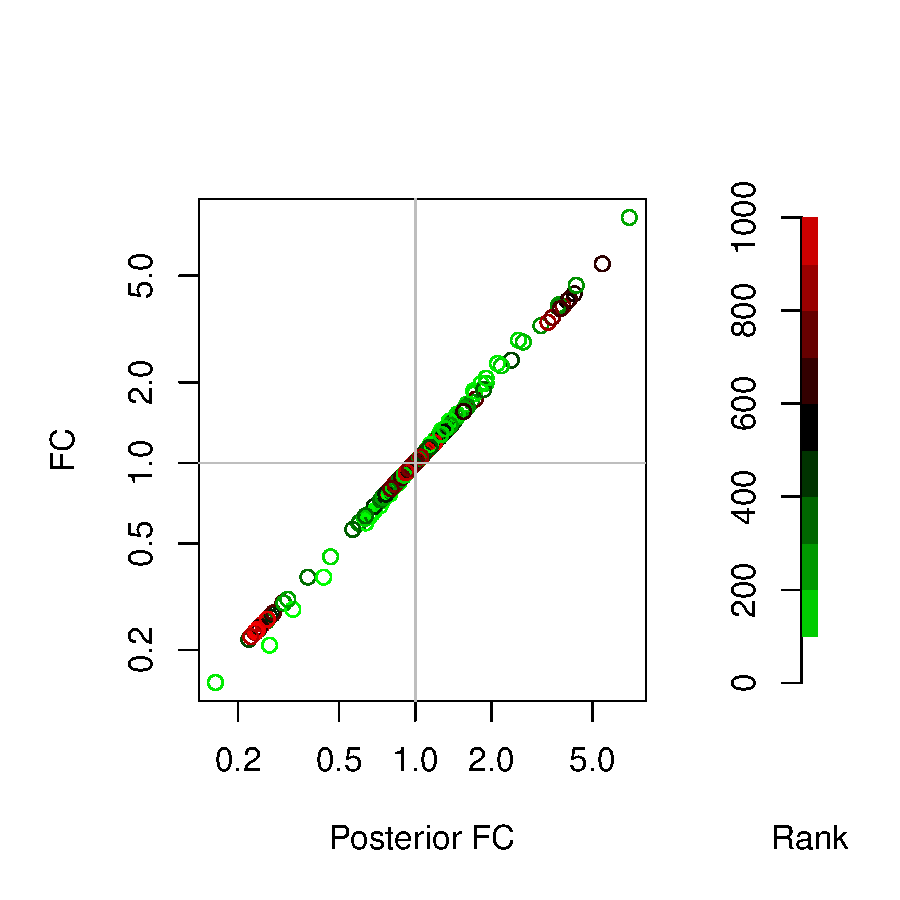
\includegraphics{EBSeq_Vignette-021}
\caption{
FC vs. Posterior FC for 1,000 gene expression estimates}
\label{fig:GeneFC}
\end{figure}
Figure \ref{fig:GeneFC} shows the FC vs. Posterior FC on 1,000 gene expression estimates. 
The genes are ranked by their cross-condition mean (adjusted by the normalization factors). 
The posterior FC tends to shrink genes with low expressions (small rank); in this case the differences
are minor. 


\newpage

\subsubsection{Checking convergence}
\label{sec:detailedgenedeconverge}
As detailed in Section \ref{sec:model}, we assume the prior distribution of $q_g^C$ is 
$Beta(\alpha,\beta)$. The EM algorithm is used to estimate the 
hyper-parameters $\alpha,\beta$ and the mixture parameter $p$. 
The optimized parameters at each iteration may be obtained as follows (recall
we are using 5 iterations for demonstration purposes): 
\begin{Schunk}
\begin{Sinput}
> EBOut$Alpha
\end{Sinput}
\begin{Soutput}
[1] 0.4064996
\end{Soutput}
\begin{Sinput}
> EBOut$Beta
\end{Sinput}
\begin{Soutput}
   [1] 1.955348 1.907624 1.954959 1.931728 1.816152 1.950997 1.947900 1.947893
   [9] 1.933258 1.935514 1.891133 1.949470 1.917977 1.954954 1.954435 1.948103
  [17] 1.940366 1.950769 1.953056 1.951891 1.786673 1.959721 1.834271 1.945084
  [25] 1.938806 1.935299 1.950782 1.957061 1.945333 1.949186 1.944042 1.946988
  [33] 1.893547 1.945252 1.935215 1.948066 1.939478 1.943912 1.953748 1.950892
  [41] 1.942371 1.951043 1.953760 1.951113 1.946312 1.951368 1.786655 1.953273
  [49] 1.866041 1.786787 1.948505 1.947872 1.887632 1.919638 1.939149 1.948350
  [57] 1.884666 1.952032 1.954719 1.853007 1.786239 1.945687 1.957861 1.957114
  [65] 1.878675 1.920783 1.784751 1.946729 1.952588 1.950544 1.949082 1.924195
  [73] 1.939560 1.955457 1.949547 1.930072 1.935659 1.951006 1.942475 1.915059
  [81] 1.951448 1.929684 1.916020 1.956184 1.946070 1.937003 1.953835 1.951598
  [89] 1.949303 1.949082 1.936941 1.958086 1.941963 1.786733 1.928526 1.953510
  [97] 1.909720 1.941461 1.919982 1.949197 1.907385 1.927028 1.890164 1.953884
 [105] 1.790063 1.942100 1.933681 1.951821 1.943492 1.959838 1.856778 1.949530
 [113] 1.956185 1.956466 1.954509 1.957701 1.896579 1.956127 1.957862 1.895715
 [121] 1.959079 1.949076 1.950701 1.789779 1.946335 1.943948 1.936897 1.949862
 [129] 1.950456 1.952377 1.790090 1.946223 1.942124 1.956934 1.951340 1.950675
 [137] 1.951398 1.935169 1.911897 1.944289 1.953257 1.958941 1.913765 1.954621
 [145] 1.945531 1.790000 1.948752 1.959761 1.956868 1.959807 1.790862 1.951776
 [153] 1.790331 1.958258 1.789975 1.918622 1.791606 1.915789 1.891709 1.789846
 [161] 1.789832 1.954432 1.959946 1.938875 1.956064 1.857600 1.959013 1.957141
 [169] 1.953433 1.959066 1.892698 1.955345 1.958690 1.789809 1.932713 1.858145
 [177] 1.959261 1.789788 1.954924 1.791453 1.952613 1.952996 1.790560 1.936941
 [185] 1.935750 1.955410 1.958287 1.921822 1.957858 1.789808 1.887722 1.956674
 [193] 1.955732 1.931640 1.790330 1.887720 1.930539 1.789785 1.957229 1.955300
 [201] 1.957335 1.938117 1.790271 1.959911 1.941475 1.957705 1.959345 1.956430
 [209] 1.955083 1.901715 1.936953 1.917350 1.950494 1.956856 1.789805 1.959481
 [217] 1.959097 1.899997 1.789912 1.790765 1.789794 1.946949 1.958608 1.935662
 [225] 1.947768 1.957341 1.944313 1.957395 1.789957 1.892023 1.933700 1.958329
 [233] 1.956122 1.957135 1.949353 1.958358 1.789839 1.924835 1.870776 1.953835
 [241] 1.790465 1.891202 1.955067 1.952179 1.952779 1.956732 1.957788 1.952728
 [249] 1.943051 1.941620 1.951246 1.949310 1.959757 1.958369 1.953623 1.958114
 [257] 1.959539 1.913905 1.957919 1.950351 1.944903 1.913535 1.953745 1.946968
 [265] 1.893228 1.790451 1.939070 1.941844 1.868482 1.928873 1.936448 1.951366
 [273] 1.933847 1.958148 1.959589 1.958425 1.947652 1.935689 1.946050 1.959858
 [281] 1.958314 1.959709 1.789780 1.949042 1.920015 1.833136 1.956261 1.948466
 [289] 1.953503 1.791890 1.956364 1.949070 1.789841 1.948079 1.958166 1.940251
 [297] 1.958311 1.951878 1.954394 1.958120 1.942443 1.929474 1.889705 1.955223
 [305] 1.928079 1.789806 1.954423 1.790270 1.900408 1.951917 1.789823 1.954204
 [313] 1.789790 1.959367 1.923076 1.954824 1.957312 1.937913 1.883757 1.958015
 [321] 1.944746 1.942133 1.958137 1.954040 1.958405 1.957659 1.952593 1.955171
 [329] 1.790214 1.952593 1.950096 1.957405 1.954803 1.853016 1.951360 1.791568
 [337] 1.955795 1.952247 1.935384 1.950304 1.953308 1.958883 1.895927 1.950320
 [345] 1.925162 1.953573 1.920457 1.959572 1.950715 1.958016 1.948624 1.958622
 [353] 1.947084 1.789896 1.921815 1.956599 1.956495 1.789984 1.949205 1.951025
 [361] 1.958040 1.790140 1.953864 1.958059 1.945530 1.933925 1.956562 1.890909
 [369] 1.913798 1.951947 1.933930 1.789866 1.909726 1.949217 1.790441 1.950032
 [377] 1.894487 1.789813 1.959294 1.946971 1.954895 1.926611 1.928539 1.789849
 [385] 1.879793 1.957181 1.824880 1.959034 1.958868 1.883909 1.952617 1.956738
 [393] 1.956520 1.931955 1.947725 1.956631 1.959241 1.950375 1.947866 1.922100
 [401] 1.946863 1.853036 1.939661 1.956583 1.790377 1.941762 1.789936 1.954746
 [409] 1.870758 1.901352 1.953739 1.946726 1.953982 1.955890 1.955926 1.948204
 [417] 1.951569 1.957854 1.789835 1.959115 1.955498 1.791363 1.931482 1.955465
 [425] 1.882136 1.943589 1.958518 1.956973 1.955993 1.948048 1.953486 1.957760
 [433] 1.943834 1.791736 1.789887 1.789849 1.922029 1.930647 1.907459 1.950444
 [441] 1.958107 1.930241 1.957892 1.789785 1.959019 1.955361 1.941099 1.955261
 [449] 1.943526 1.946957 1.790165 1.919363 1.957937 1.907867 1.947910 1.925102
 [457] 1.931279 1.949964 1.946249 1.942683 1.948231 1.955430 1.790204 1.786254
 [465] 1.944392 1.955640 1.790306 1.959389 1.952874 1.959444 1.951089 1.939537
 [473] 1.951204 1.946427 1.957743 1.789832 1.951552 1.792651 1.903203 1.921007
 [481] 1.955522 1.880634 1.937185 1.948166 1.948517 1.960089 1.958043 1.958681
 [489] 1.952286 1.922313 1.953857 1.958561 1.958291 1.789803 1.956617 1.945902
 [497] 1.955610 1.955934 1.958123 1.954809 1.953177 1.946948 1.940024 1.959409
 [505] 1.872064 1.956973 1.947238 1.883682 1.948128 1.909649 1.951769 1.958135
 [513] 1.889836 1.945813 1.924382 1.932743 1.791511 1.932406 1.943079 1.883620
 [521] 1.935521 1.918838 1.920154 1.942491 1.957003 1.954219 1.792733 1.932373
 [529] 1.789890 1.959438 1.959444 1.955800 1.937502 1.855334 1.957795 1.878686
 [537] 1.953415 1.949118 1.945512 1.954937 1.957051 1.957880 1.954287 1.944747
 [545] 1.955127 1.953520 1.958502 1.949488 1.791531 1.902028 1.928528 1.955434
 [553] 1.927376 1.946744 1.957619 1.957985 1.789790 1.789779 1.958392 1.924895
 [561] 1.958237 1.959501 1.952860 1.790366 1.958216 1.957801 1.959805 1.958956
 [569] 1.902355 1.883014 1.953340 1.957644 1.861285 1.955539 1.789783 1.953864
 [577] 1.951815 1.883282 1.956375 1.913237 1.958834 1.944428 1.955860 1.790333
 [585] 1.956355 1.954415 1.959147 1.892547 1.954612 1.955654 1.790084 1.955471
 [593] 1.875581 1.790376 1.947831 1.952559 1.939973 1.791760 1.956328 1.946115
 [601] 1.959327 1.944510 1.947234 1.945165 1.941634 1.926492 1.930426 1.958365
 [609] 1.950823 1.957090 1.926532 1.911564 1.956083 1.789977 1.957903 1.959793
 [617] 1.958005 1.789952 1.952390 1.935208 1.957404 1.956906 1.789805 1.950646
 [625] 1.941700 1.957929 1.789792 1.937014 1.945091 1.955878 1.937998 1.959928
 [633] 1.878079 1.950391 1.958215 1.959048 1.931988 1.953369 1.958675 1.789810
 [641] 1.790218 1.949465 1.903102 1.955545 1.949540 1.952957 1.790330 1.945226
 [649] 1.945529 1.927116 1.890921 1.959076 1.953342 1.789775 1.932824 1.957393
 [657] 1.955187 1.956190 1.868923 1.938150 1.957263 1.955935 1.948461 1.954935
 [665] 1.956882 1.955595 1.945041 1.942455 1.958885 1.951449 1.944788 1.789780
 [673] 1.789849 1.789915 1.945998 1.948288 1.949347 1.954057 1.955875 1.942903
 [681] 1.957101 1.951815 1.922952 1.948830 1.789803 1.951718 1.947875 1.951319
 [689] 1.955753 1.954324 1.933395 1.955526 1.940220 1.952657 1.955657 1.784079
 [697] 1.941511 1.791018 1.951578 1.955733 1.952148 1.956801 1.959850 1.954337
 [705] 1.950900 1.923664 1.791296 1.931685 1.957920 1.955501 1.954119 1.938754
 [713] 1.959996 1.942738 1.898091 1.959307 1.936465 1.789782 1.950664 1.948960
 [721] 1.957818 1.953349 1.954956 1.956551 1.789794 1.948931 1.951123 1.953940
 [729] 1.934787 1.897844 1.778873 1.958575 1.943358 1.945574 1.899622 1.953143
 [737] 1.957672 1.956913 1.957096 1.954008 1.951484 1.934516 1.958586 1.948599
 [745] 1.950953 1.942406 1.955221 1.959235 1.950717 1.954833 1.959636 1.910026
 [753] 1.955479 1.932504 1.938506 1.933706 1.952101 1.957483 1.939835 1.917287
 [761] 1.958033 1.898404 1.789784 1.951120 1.952009 1.949620 1.956581 1.956745
 [769] 1.926319 1.789974 1.958246 1.953251 1.941275 1.953022 1.956243 1.955107
 [777] 1.897031 1.948103 1.867493 1.957197 1.789783 1.956533 1.955946 1.948934
 [785] 1.929796 1.878456 1.950291 1.959224 1.956177 1.958436 1.944770 1.945937
 [793] 1.957667 1.959295 1.956113 1.937309 1.955738 1.954053 1.958956 1.952927
 [801] 1.956762 1.873459 1.940529 1.940074 1.958631 1.903894 1.953113 1.789788
 [809] 1.790322 1.876944 1.956957 1.942427 1.925936 1.946719 1.943941 1.789836
 [817] 1.941335 1.935198 1.942957 1.958173 1.789890 1.959609 1.958605 1.959530
 [825] 1.949007 1.953889 1.953237 1.936824 1.928975 1.939681 1.947936 1.956086
 [833] 1.789803 1.957676 1.953171 1.930152 1.936353 1.951487 1.935013 1.958810
 [841] 1.937513 1.953297 1.958237 1.948185 1.789836 1.949631 1.790129 1.955794
 [849] 1.955838 1.945287 1.940669 1.954590 1.901307 1.922020 1.952343 1.948252
 [857] 1.840985 1.953435 1.789979 1.957961 1.936172 1.954502 1.926417 1.940044
 [865] 1.955356 1.947220 1.959233 1.957745 1.790136 1.790511 1.955547 1.957582
 [873] 1.934678 1.959904 1.958751 1.905192 1.945692 1.865177 1.952916 1.930768
 [881] 1.959216 1.947176 1.952798 1.792784 1.952415 1.955214 1.959012 1.943531
 [889] 1.924320 1.933510 1.951822 1.944066 1.790036 1.954296 1.951999 1.937551
 [897] 1.954920 1.790788 1.954278 1.942559 1.959418 1.953685 1.956582 1.938347
 [905] 1.956443 1.949294 1.954962 1.953599 1.936559 1.958189 1.945121 1.928619
 [913] 1.940776 1.940486 1.959321 1.956046 1.955112 1.959094 1.957251 1.917096
 [921] 1.957236 1.917472 1.958974 1.941602 1.954892 1.948363 1.949077 1.958125
 [929] 1.958253 1.954183 1.792279 1.954436 1.824686 1.789790 1.959873 1.940255
 [937] 1.959137 1.789994 1.949142 1.952876 1.891903 1.950896 1.949804 1.946816
 [945] 1.959425 1.956947 1.790078 1.949934 1.955840 1.957698 1.938980 1.953376
 [953] 1.949468 1.789854 1.940750 1.953619 1.954402 1.933773 1.957474 1.934070
 [961] 1.953238 1.957120 1.918998 1.953527 1.789789 1.946928 1.949293 1.863585
 [969] 1.911040 1.948184 1.949035 1.761709 1.952436 1.952580 1.939440 1.915143
 [977] 1.942051 1.958989 1.789781 1.789915 1.951986 1.790663 1.943799 1.857008
 [985] 1.955058 1.791165 1.789789 1.951860 1.931629 1.939894 1.957231 1.957450
 [993] 1.910961 1.894587 1.959008 1.959129 1.957413 1.789772 1.901920 1.959698
\end{Soutput}
\begin{Sinput}
> EBOut$P
\end{Sinput}
\begin{Soutput}
[1] 0.1082901 0.8917099
\end{Soutput}
\end{Schunk}
In this case the differences between the 4th and 5th iterations are always less 
than 0.01.


\subsubsection{Checking the model fit and other diagnostics}
\label{sec:detailedgenedeplot}
As noted in Leng {\it et al.}, 2013 \cite{Leng13}, EBSeq relies on parametric assumptions that should
be checked following each analysis.
The \verb+QQP+ function may be used to assess prior assumptions. 
In practice, \verb+QQP+ generates the Q-Q plot of the empirical $q$'s 
vs. the simulated $q$'s from the Beta prior distribution with 
estimated hyper-parameters. Figure \ref{fig:GeneQQ} shows that the 
data points lie on the $y=x$ line for both conditions, which indicates 
that the Beta prior is appropriate.

\begin{figure}[h!]
\centering
\begin{Schunk}
\begin{Sinput}
> par(mfrow=c(1,2))
> QQP(EBOut)
\end{Sinput}
\end{Schunk}
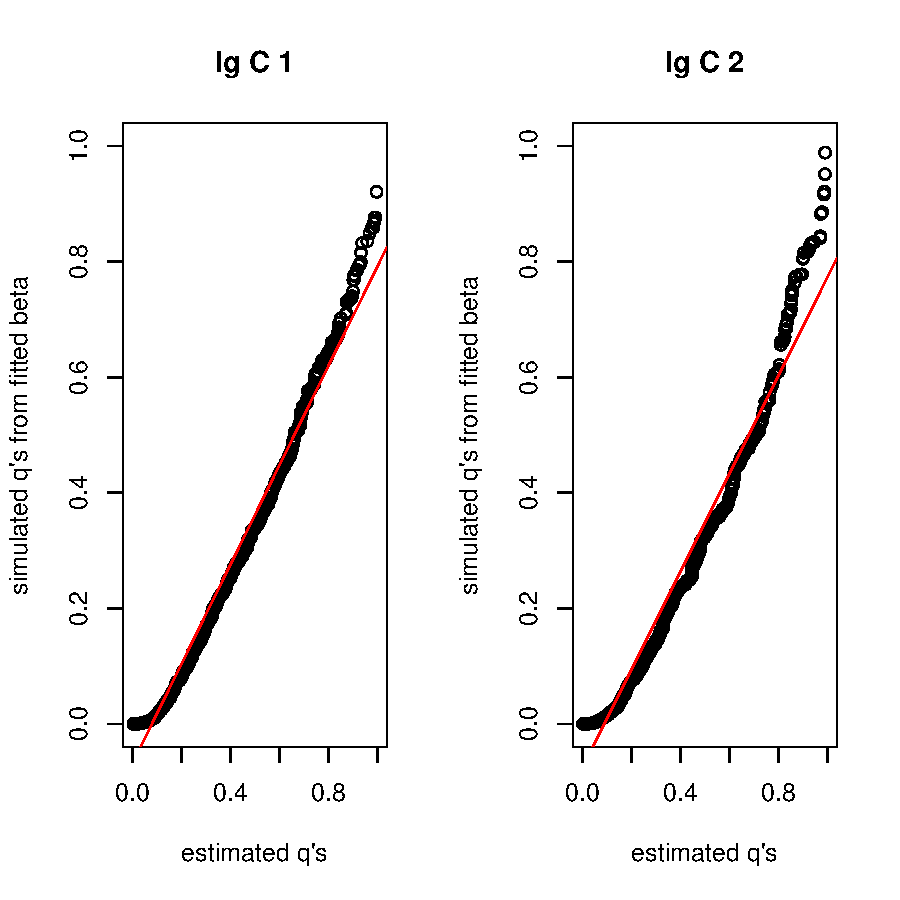
\includegraphics{EBSeq_Vignette-023}
\caption{QQ-plots for checking the assumption of a Beta prior (upper panels) as well as the
model fit using data from condition 1 and condition 2 (lower panels)}
\label{fig:GeneQQ}
\end{figure}

\newpage
\noindent  
Likewise, the \verb+DenNHist+ function may be used to check the density plot of empirical $q$'s vs the simulated
$q$'s from the fitted Beta prior distribution. 
Figure \ref{fig:GeneDenNHist} also shows our estimated distribution fits the 
data very well.

\begin{figure}[h!]
\centering
\begin{Schunk}
\begin{Sinput}
> par(mfrow=c(1,2))
> DenNHist(EBOut)
\end{Sinput}
\end{Schunk}
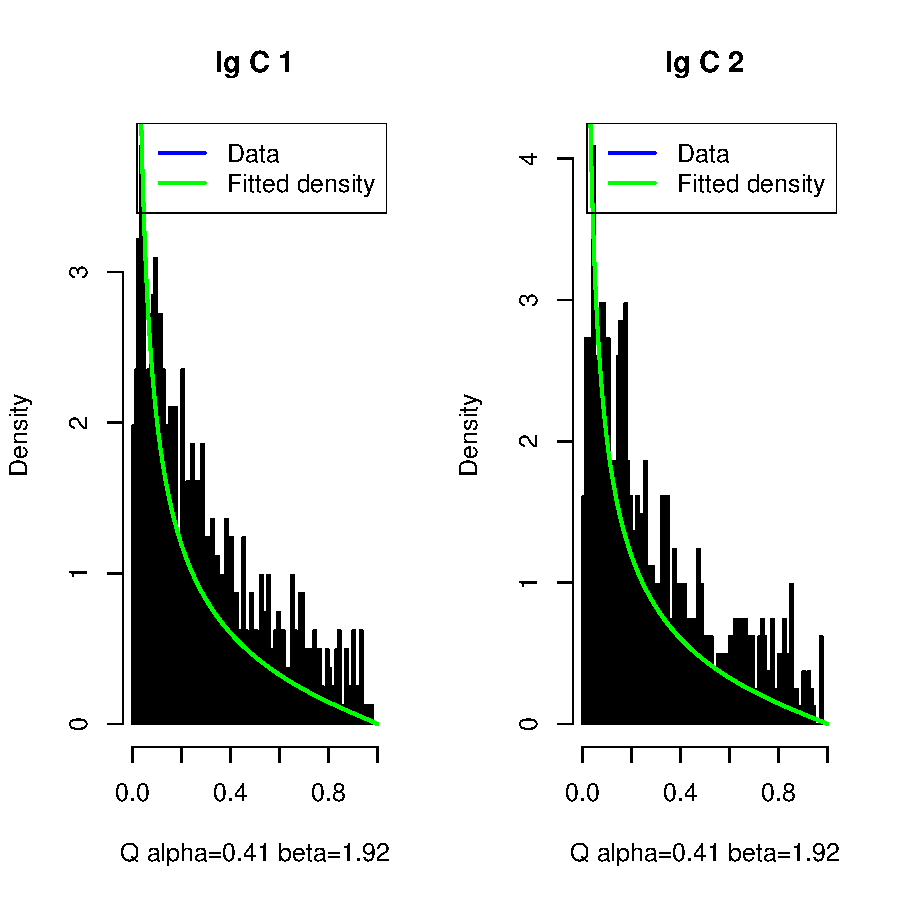
\includegraphics{EBSeq_Vignette-024}
\caption{Density plots for checking the model fit using data from condition 1 and condition 2}
\label{fig:GeneDenNHist}
\end{figure}

\newpage
\subsection{Isoform level DE analysis (two conditions)}
\label{sec:detailedisode}
\subsubsection{The $I_g$ vector}
\label{sec:detailedisodeNg}
Since EBSeq fits rely on $I_g$, 
we need to obtain the $I_g$ for each isoform. This can be done using the 
function \verb+GetNg+. 
The required inputs of \verb+GetNg+ are the isoform names (\verb+IsoformNames+) and 
their corresponding gene names (\verb+IsosGeneNames+), described above.
In the simulated data, we assume that the isoforms in the $I_g=1$ group belong to genes \verb+Gene_1, ... , Gene_200+; 
The isoforms in the $I_g=2$ group belong to genes 
\verb+Gene_201, ..., Gene_400+; and isoforms in the $I_g=3$ group 
belong to \verb+Gene_401, ..., Gene_600+.

\begin{Schunk}
\begin{Sinput}
> data(IsoList)
> IsoMat=IsoList$IsoMat
> IsoNames=IsoList$IsoNames
> IsosGeneNames=IsoList$IsosGeneNames
> NgList=GetNg(IsoNames, IsosGeneNames, TrunThre=3)
\end{Sinput}
\end{Schunk}
\begin{Schunk}
\begin{Sinput}
> names(NgList)
\end{Sinput}
\begin{Soutput}
[1] "GeneNg"        "GeneNgTrun"    "IsoformNg"     "IsoformNgTrun"
\end{Soutput}
\begin{Sinput}
> IsoNgTrun=NgList$IsoformNgTrun
> IsoNgTrun[c(1:3,201:203,601:603)]
\end{Sinput}
\begin{Soutput}
Iso_1_1 Iso_1_2 Iso_1_3 Iso_2_1 Iso_2_2 Iso_2_3 Iso_3_1 Iso_3_2 Iso_3_3 
      1       1       1       2       2       2       3       3       3 
\end{Soutput}
\end{Schunk}

The output of \verb+GetNg+ contains 4 vectors. \verb+GeneNg+ (\verb+IsoformNg+) provides 
the number of isoforms $N_g$ within each gene (within each isoform's host gene). 
\verb+GeneNgTrun+ (\verb+IsoformNgTrun+) provides the $I_g$ group assignments. 
The default number of groups is 3, which means the isoforms  
with $N_g$  greater than 3 will be assigned to $I_g=3$ group.
We use 3 in the case studies 
since the number of isoforms with $N_g$ larger than 3 is relatively small and 
the small sample size may induce poor parameter fitting if we treat them 
as separate groups.  
In practice, if there is evidence that the $N_g=4,5,6...$ groups should be 
treated as separate groups, a user can change \verb+TrunThre+ to define 
a different truncation threshold.

\subsubsection{Using mappability ambiguity clusters instead of 
the $I_g$ vector when the gene-isoform relationship is unknown}
\label{sec:detailedisodeNoNg}
When working with a de-novo assembled transcriptome, in which case the gene-isoform 
relationship is unknown, 
a user can use read mapping ambiguity cluster information instead of Ng,
as provided by RSEM \cite{Li11b} in the
output file \verb+output_name.ngvec+. The file contains a vector with the same 
length as the total number of transcripts. 
Each transcript has been assigned to one of 3 levels 
(1, 2, or 3) to indicate the mapping uncertainty level of that transcript. 
The mapping ambiguity clusters are partitioned via a k-means algorithm on the unmapability 
scores that are provided by RSEM.  A user can read in the mapping ambiguity cluster information  
using:

\begin{Schunk}
\begin{Sinput}
> IsoNgTrun = scan(file="output_name.ngvec", what=0, sep="\n")
\end{Sinput}
\end{Schunk}
Where \verb+"output_name.ngvec"+ is the output file obtained from RSEM function rsem-generate-ngvector. 
More details on using the RSEM-EBSeq pipeline 
on de novo assembled transcriptomes can be found 
at \url{http://deweylab.biostat.wisc.edu/rsem/README.html#de}.

Other unmappability scores and other cluster methods (e.g. Gaussian Mixed Model) 
could also be used to form the uncertainty clusters.

\subsubsection{Running EBSeq on simulated isoform expression estimates}
\label{sec:detailedisoderun}
EBSeq can be applied as described in Section \ref{sec:startisoderun}.
\begin{Schunk}
\begin{Sinput}
> IsoSizes=MedianNorm(IsoMat)
> IsoEBOut=EBTest(Data=IsoMat, NgVector=IsoNgTrun, 
+ Conditions=as.factor(rep(c("C1","C2"),each=5)),sizeFactors=IsoSizes)
> IsoEBDERes=GetDEResults(IsoEBOut, FDR=0.05)
\end{Sinput}
\end{Schunk}
\begin{Schunk}
\begin{Sinput}
> str(IsoEBDERes)
\end{Sinput}
\begin{Soutput}
List of 3
 $ DEfound: chr [1:104] "Iso_1_1" "Iso_1_2" "Iso_1_3" "Iso_1_4" ...
 $ PPMat  : num [1:1200, 1:2] 1.18e-18 2.44e-83 0.00 5.59e-206 3.90e-71 ...
  ..- attr(*, "dimnames")=List of 2
  .. ..$ : chr [1:1200] "Iso_1_1" "Iso_1_2" "Iso_1_3" "Iso_1_4" ...
  .. ..$ : chr [1:2] "PPEE" "PPDE"
 $ Status : Named chr [1:1200] "DE" "DE" "DE" "DE" ...
  ..- attr(*, "names")= chr [1:1200] "Iso_1_1" "Iso_1_2" "Iso_1_3" "Iso_1_4" ...
\end{Soutput}
\end{Schunk}
\noindent We see that EBSeq found 104 DE isoforms at a target FDR of 0.05. 
The function \verb+PostFC+ could also be used here to calculate the Fold Change (FC) 
as well as the posterior FC on the normalization factor adjusted data.
\begin{Schunk}
\begin{Sinput}
> IsoFC=PostFC(IsoEBOut)
> str(IsoFC)
\end{Sinput}
\begin{Soutput}
List of 3
 $ PostFC   : num [1:1200, 1] 0.286 0.281 3.553 0.305 3.755 ...
 $ RealFC   : Named num [1:1200] 0.285 0.281 3.556 0.305 3.759 ...
  ..- attr(*, "names")= chr [1:1200] "Iso_1_1" "Iso_1_2" "Iso_1_3" "Iso_1_4" ...
 $ Direction: chr "C1 Over C2"
\end{Soutput}
\end{Schunk}


\subsubsection{Checking convergence}
\label{sec:detailedisodeconverge}
For isoform level data, we assume the prior distribution of $q_{gi}^C$ is
$Beta(\alpha,\beta^{I_g})$.
As in Section \ref{sec:detailedgenedeconverge}, the optimized parameters at each iteration 
may be obtained as follows (recall
we are using 5 iterations for demonstration purposes): 
\begin{Schunk}
\begin{Sinput}
> IsoEBOut$Alpha
\end{Sinput}
\begin{Soutput}
[1] 0.405096
\end{Soutput}
\begin{Sinput}
> IsoEBOut$Beta
\end{Sinput}
\begin{Soutput}
   [1] 2 2 2 2 2 2 2 2 2 2 2 2 2 2 2 2 2 2 2 2 2 2 2 2 2 2 2 2 2 2 2 2 2 2 2 2 2
  [38] 2 2 2 2 2 2 2 2 2 2 2 2 2 2 2 2 2 2 2 2 2 2 2 2 2 2 2 2 2 2 2 2 2 2 2 2 2
  [75] 2 2 2 2 2 2 2 2 2 2 2 2 2 2 2 2 2 2 2 2 2 2 2 2 2 2 2 2 2 2 2 2 2 2 2 2 2
 [112] 2 2 2 2 2 2 2 2 2 2 2 2 2 2 2 2 2 2 2 2 2 2 2 2 2 2 2 2 2 2 2 2 2 2 2 2 2
 [149] 2 2 2 2 2 2 2 2 2 2 2 2 2 2 2 2 2 2 2 2 2 2 2 2 2 2 2 2 2 2 2 2 2 2 2 2 2
 [186] 2 2 2 2 2 2 2 2 2 2 2 2 2 2 2 2 2 2 2 2 2 2 2 2 2 2 2 2 2 2 2 2 2 2 2 2 2
 [223] 2 2 2 2 2 2 2 2 2 2 2 2 2 2 2 2 2 2 2 2 2 2 2 2 2 2 2 2 2 2 2 2 2 2 2 2 2
 [260] 2 2 2 2 2 2 2 2 2 2 2 2 2 2 2 2 2 2 2 2 2 2 2 2 2 2 2 2 2 2 2 2 2 2 2 2 2
 [297] 2 2 2 2 2 2 2 2 2 2 2 2 2 2 2 2 2 2 2 2 2 2 2 2 2 2 2 2 2 2 2 2 2 2 2 2 2
 [334] 2 2 2 2 2 2 2 2 2 2 2 2 2 2 2 2 2 2 2 2 2 2 2 2 2 2 2 2 2 2 2 2 2 2 2 2 2
 [371] 2 2 2 2 2 2 2 2 2 2 2 2 2 2 2 2 2 2 2 2 2 2 2 2 2 2 2 2 2 2 2 2 2 2 2 2 2
 [408] 2 2 2 2 2 2 2 2 2 2 2 2 2 2 2 2 2 2 2 2 2 2 2 2 2 2 2 2 2 2 2 2 2 2 2 2 2
 [445] 2 2 2 2 2 2 2 2 2 2 2 2 2 2 2 2 2 2 2 2 2 2 2 2 2 2 2 2 2 2 2 2 2 2 2 2 2
 [482] 2 2 2 2 2 2 2 2 2 2 2 2 2 2 2 2 2 2 2 2 2 2 2 2 2 2 2 2 2 2 2 2 2 2 2 2 2
 [519] 2 2 2 2 2 2 2 2 2 2 2 2 2 2 2 2 2 2 2 2 2 2 2 2 2 2 2 2 2 2 2 2 2 2 2 2 2
 [556] 2 2 2 2 2 2 2 2 2 2 2 2 2 2 2 2 2 2 2 2 2 2 2 2 2 2 2 2 2 2 2 2 2 2 2 2 2
 [593] 2 2 2 2 2 2 2 2 2 2 2 2 2 2 2 2 2 2 2 2 2 2 2 2 2 2 2 2 2 2 2 2 2 2 2 2 2
 [630] 2 2 2 2 2 2 2 2 2 2 2 2 2 2 2 2 2 2 2 2 2 2 2 2 2 2 2 2 2 2 2 2 2 2 2 2 2
 [667] 2 2 2 2 2 2 2 2 2 2 2 2 2 2 2 2 2 2 2 2 2 2 2 2 2 2 2 2 2 2 2 2 2 2 2 2 2
 [704] 2 2 2 2 2 2 2 2 2 2 2 2 2 2 2 2 2 2 2 2 2 2 2 2 2 2 2 2 2 2 2 2 2 2 2 2 2
 [741] 2 2 2 2 2 2 2 2 2 2 2 2 2 2 2 2 2 2 2 2 2 2 2 2 2 2 2 2 2 2 2 2 2 2 2 2 2
 [778] 2 2 2 2 2 2 2 2 2 2 2 2 2 2 2 2 2 2 2 2 2 2 2 2 2 2 2 2 2 2 2 2 2 2 2 2 2
 [815] 2 2 2 2 2 2 2 2 2 2 2 2 2 2 2 2 2 2 2 2 2 2 2 2 2 2 2 2 2 2 2 2 2 2 2 2 2
 [852] 2 2 2 2 2 2 2 2 2 2 2 2 2 2 2 2 2 2 2 2 2 2 2 2 2 2 2 2 2 2 2 2 2 2 2 2 2
 [889] 2 2 2 2 2 2 2 2 2 2 2 2 2 2 2 2 2 2 2 2 2 2 2 2 2 2 2 2 2 2 2 2 2 2 2 2 2
 [926] 2 2 2 2 2 2 2 2 2 2 2 2 2 2 2 2 2 2 2 2 2 2 2 2 2 2 2 2 2 2 2 2 2 2 2 2 2
 [963] 2 2 2 2 2 2 2 2 2 2 2 2 2 2 2 2 2 2 2 2 2 2 2 2 2 2 2 2 2 2 2 2 2 2 2 2 2
[1000] 2 2 2 2 2 2 2 2 2 2 2 2 2 2 2 2 2 2 2 2 2 2 2 2 2 2 2 2 2 2 2 2 2 2 2 2 2
[1037] 2 2 2 2 2 2 2 2 2 2 2 2 2 2 2 2 2 2 2 2 2 2 2 2 2 2 2 2 2 2 2 2 2 2 2 2 2
[1074] 2 2 2 2 2 2 2 2 2 2 2 2 2 2 2 2 2 2 2 2 2 2 2 2 2 2 2 2 2 2 2 2 2 2 2 2 2
[1111] 2 2 2 2 2 2 2 2 2 2 2 2 2 2 2 2 2 2 2 2 2 2 2 2 2 2 2 2 2 2 2 2 2 2 2 2 2
[1148] 2 2 2 2 2 2 2 2 2 2 2 2 2 2 2 2 2 2 2 2 2 2 2 2 2 2 2 2 2 2 2 2 2 2 2 2 2
[1185] 2 2 2 2 2 2 2 2 2 2 2 2 2 2 2 2
\end{Soutput}
\begin{Sinput}
> IsoEBOut$P
\end{Sinput}
\begin{Soutput}
[1] 0.1175121 0.8824879
\end{Soutput}
\end{Schunk}
Here we have 3 $\beta$'s in each iteration corresponding to 
$\beta^{I_g=1},\beta^{I_g=2},\beta^{I_g=3}$.
We see that parameters are changing less than $10^{-2}$ or $10^{-3}$.
In practice, we require changes less than $10^{-3}$ to declare convergence.

\subsubsection{Checking the model fit and other diagnostics}
\label{sec:detailedisodeplot}
In Leng {\it et al.}, 2013\citep{Leng13}, we showed the mean-variance differences across different 
isoform groups on multiple data sets. 
In practice, if it is of interest to check differences among 
isoform groups defined by truncated $I_g$ (such as those shown here
in Figure 1), the function \verb+PolyFitPlot+ may be used. 
The following code generates the three
panels shown in Figure \ref{fig:IsoSimuNgEach}
(if condition 2 is of interest, a user could change each \verb+group = 1 + to \verb+group = 2+.):
\begin{figure}[h!]
\centering
\begin{Schunk}
\begin{Sinput}
> par(mfrow=c(2,2))
> PolyFitValue=vector("list",3)
> for(i in 1:3){
+   group = 1
+   PolyFitValue[[i]]=PolyFitPlot(IsoEBOut$Mean[which(IsoEBOut$Iso == i),group], 
+     IsoEBOut$Var[which(IsoEBOut$Iso == i),group],5)
+ }
>     
\end{Sinput}
\end{Schunk}
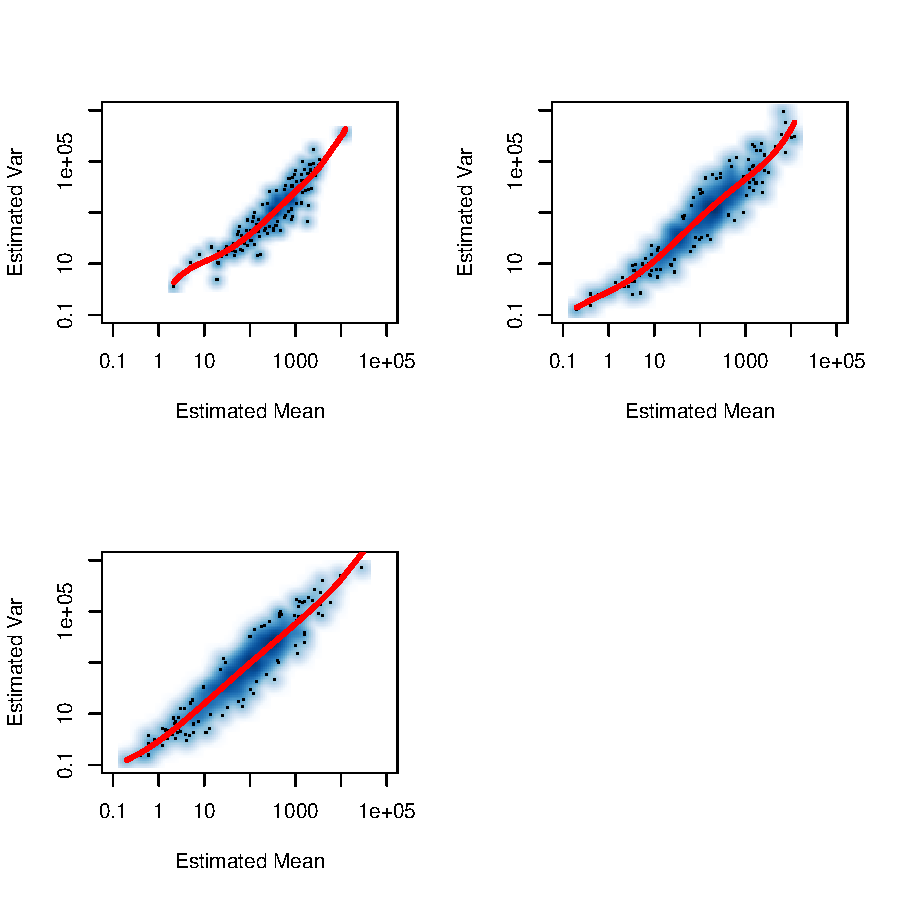
\includegraphics{EBSeq_Vignette-032}
\caption{ The mean-variance fitting plot for each Ng group}
\label{fig:IsoSimuNgEach}
\end{figure}

\newpage
Superimposing all $I_g$ groups using the code below will generate the figure (shown 
here in Figure \ref{fig:IsoSimuNg}), which is similar in structure to Figure 1:


\begin{figure}[h!]
\centering
\begin{Schunk}
\begin{Sinput}
> group = 1
> X = IsoEBOut$Mean[,group]
> Y = IsoEBOut$Var[,group]
> PolyAll=PolyFitPlot(X, Y,5)
> lines(log10(X[which(IsoEBOut$Iso == 1)][PolyFitValue[[1]]$sort]), 
+ PolyFitValue[[1]]$fit[PolyFitValue[[1]]$sort],col="yellow",lwd=2)
> lines(log10(X[which(IsoEBOut$Iso == 2)][PolyFitValue[[2]]$sort]), 
+ PolyFitValue[[2]]$fit[PolyFitValue[[2]]$sort],col="pink",lwd=2)
> lines(log10(X[which(IsoEBOut$Iso == 3)][PolyFitValue[[3]]$sort]), 
+ PolyFitValue[[3]]$fit[PolyFitValue[[3]]$sort],col="green",lwd=2)
> legend("topleft",c("All Isoforms","Ng = 1","Ng = 2","Ng = 3"),
+ col=c("red","yellow","pink","green"),lty=1,lwd=3,box.lwd=2)
\end{Sinput}
\end{Schunk}
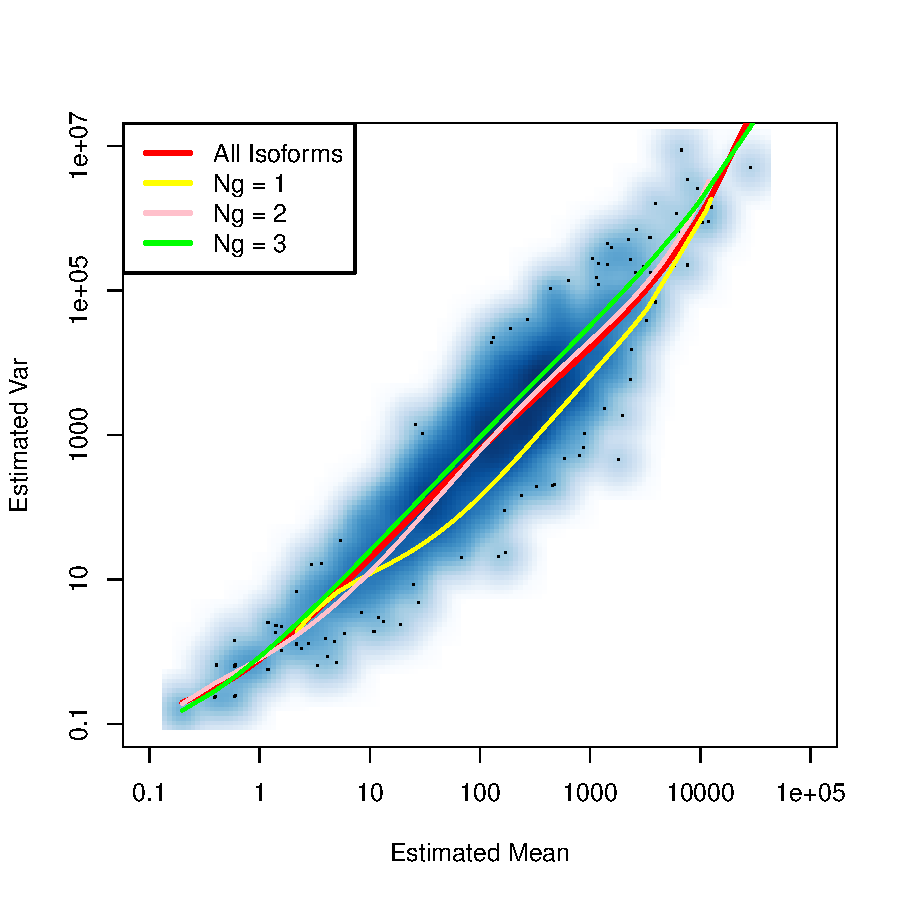
\includegraphics{EBSeq_Vignette-033}
\caption{The mean-variance plot for each Ng group}
\label{fig:IsoSimuNg}
\end{figure}


\newpage
\noindent To generate a QQ-plot of the fitted Beta prior distribution 
and the $\hat{q}^C$'s within condition, a user may 
use the following code to generate 6 panels (as shown in Figure \ref{fig:IsoQQ}).
\begin{figure}[h!]
\centering
\begin{Schunk}
\begin{Sinput}
> par(mfrow=c(2,3))
> QQP(IsoEBOut)
\end{Sinput}
\end{Schunk}
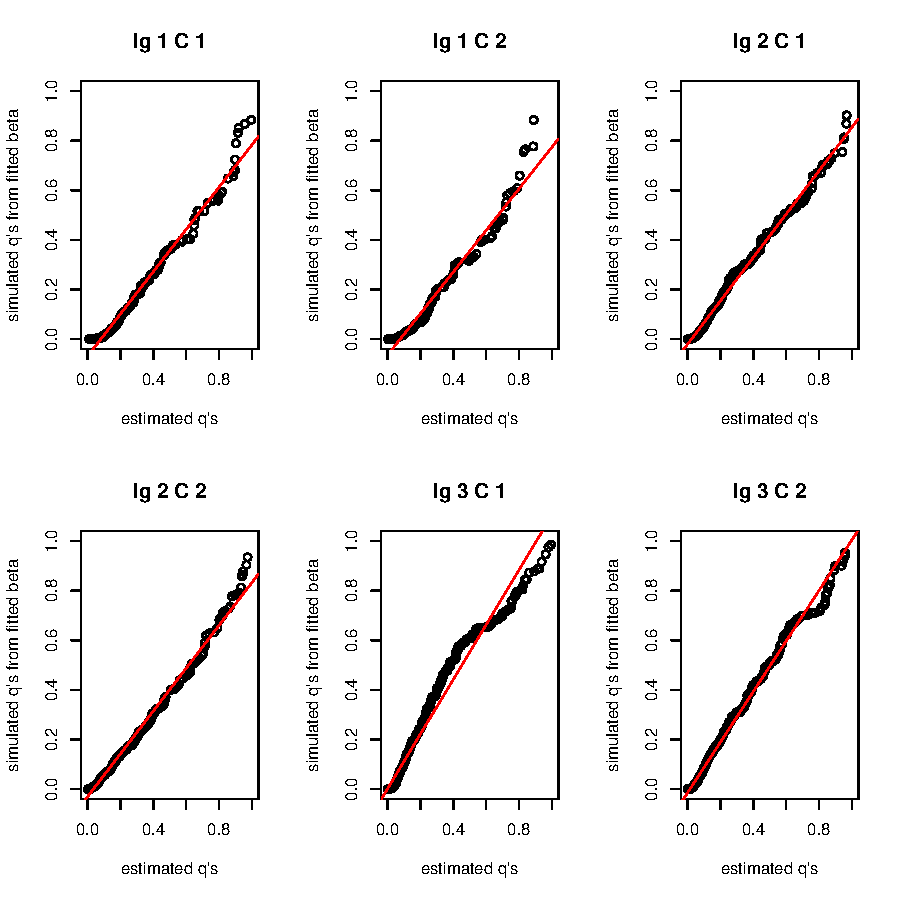
\includegraphics{EBSeq_Vignette-034}
\caption{ QQ-plots of the fitted prior distributions within each condition and each Ig group}
\label{fig:IsoQQ}
\end{figure}

\newpage
\noindent And in order to produce the plot of the fitted Beta prior densities
and the histograms of $\hat{q}^C$'s within each condition, 
the following may be used (it generates Figure \ref{fig:IsoDenNHist}):
\begin{figure}[h]
\centering
\begin{Schunk}
\begin{Sinput}
> par(mfrow=c(2,3))
> DenNHist(IsoEBOut)
\end{Sinput}
\end{Schunk}
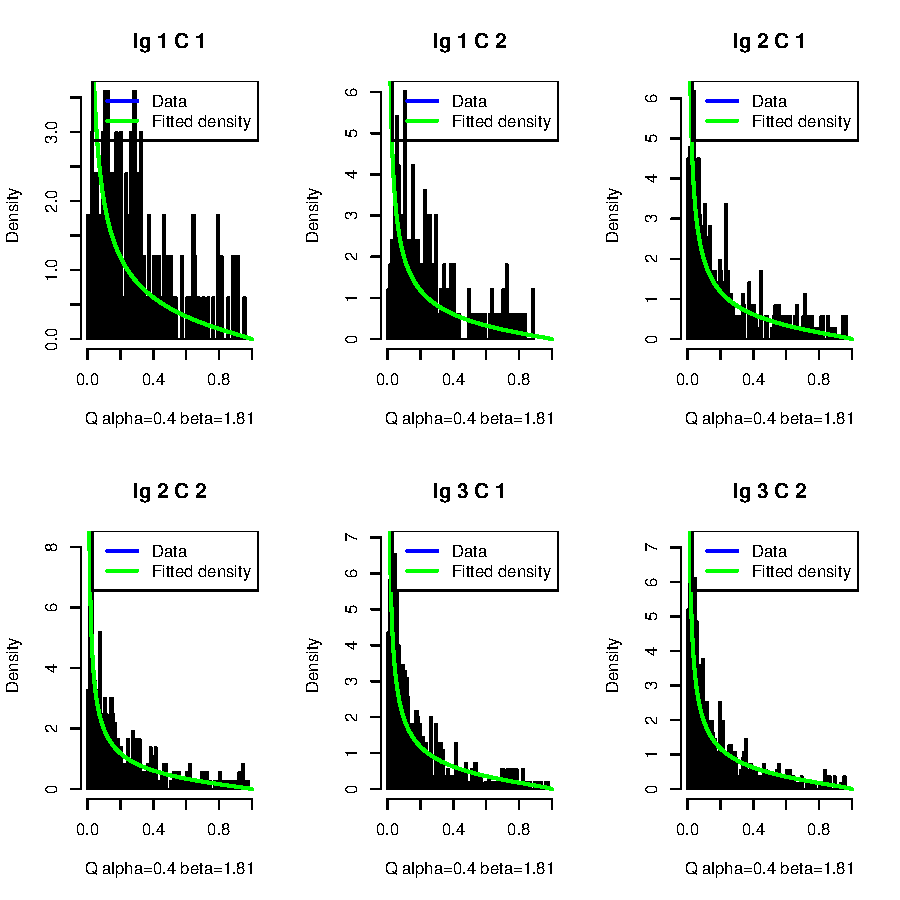
\includegraphics{EBSeq_Vignette-035}
\caption{ Prior distribution fit within each condition and each Ig group.
(Note only a small set of isoforms are considered here for demonstration.
Better fitting should be expected while using full set of isoforms.)}
\label{fig:IsoDenNHist}
\end{figure}

\clearpage
\subsection{Gene level DE analysis (more than two conditions)}
\label{sec:detailedmulticond}
\noindent 
\verb+MedianNorm+ or one of its competitors should be used to determine the normalization factors.
Once this is done, the formal test is performed by \verb+EBMultiTest+. 
\begin{Schunk}
\begin{Sinput}
> data(MultiGeneMat)
> Conditions=c("C1","C1","C2","C2","C3","C3")
> MultiSize=MedianNorm(MultiGeneMat)
> MultiOut=EBMultiTest(MultiGeneMat,
+ NgVector=NULL,Conditions=Conditions,
+ sizeFactors=MultiSize, uc = 2)
\end{Sinput}
\end{Schunk}
\noindent The posterior probability of being in each pattern for every gene is obtained using the 
function \verb+GetMultiPP+:
\begin{Schunk}
\begin{Sinput}
> MultiPP=GetMultiPP(MultiOut)
> names(MultiPP)
\end{Sinput}
\begin{Soutput}
[1] "PP"       "MAP"      "Patterns"
\end{Soutput}
\begin{Sinput}
> MultiPP$PP[1:10,]
\end{Sinput}
\begin{Soutput}
           pattern1  pattern2      pattern3      pattern4      pattern5
Gene_1  0.342709563 0.6572904  6.870408e-72  3.015440e-93  2.864790e-55
Gene_3  0.006595105 0.9934049 5.340316e-109 3.433672e-163 2.922145e-116
Gene_5  0.042482476 0.9575175  5.309949e-20  7.837887e-26  1.140460e-18
Gene_7  0.157609361 0.8423906  0.000000e+00  0.000000e+00 2.905691e-294
Gene_9  0.040619174 0.9593808  2.441999e-15  9.088562e-16  9.343836e-16
Gene_11 0.053841782 0.9461582  2.607784e-12  2.955394e-11  4.570651e-11
Gene_13 0.106486219 0.8935129  9.194008e-10  6.798796e-08  7.735994e-07
Gene_15 0.027054430 0.9729456  1.079379e-40  5.379139e-47  2.410435e-44
Gene_17 0.181376143 0.8186239 4.590012e-133 7.310837e-184 9.831129e-113
Gene_19 0.048700449 0.9512996  1.080862e-24  2.792245e-37  6.753301e-28
\end{Soutput}
\begin{Sinput}
> MultiPP$MAP[1:10]
\end{Sinput}
\begin{Soutput}
    Gene_1     Gene_3     Gene_5     Gene_7     Gene_9    Gene_11    Gene_13 
"pattern2" "pattern2" "pattern2" "pattern2" "pattern2" "pattern2" "pattern2" 
   Gene_15    Gene_17    Gene_19 
"pattern2" "pattern2" "pattern2" 
\end{Soutput}
\begin{Sinput}
> MultiPP$Patterns
\end{Sinput}
\begin{Soutput}
         C1 C2 C3
Pattern1  1  2  3
Pattern2  1  1  2
Pattern3  1  2  2
Pattern4  1  1  1
Pattern5  1  2  1
\end{Soutput}
\end{Schunk}
As described in Section \ref{sec:startmulticond}, 
the function \verb+GetPatterns+ allows the user to get selected patterns after we run the \verb+EBMultiTest+ function
To visualize the patterns, the function \verb+PlotPattern+ may be used.

\begin{figure}[h!]
\centering
\begin{Schunk}
\begin{Sinput}
> PosParti=GetPatterns(MultiOut)
> PosParti
\end{Sinput}
\begin{Soutput}
         C1 C2 C3
Pattern1  1  2  3
Pattern2  1  1  2
Pattern3  1  2  2
Pattern4  1  1  1
Pattern5  1  2  1
\end{Soutput}
\begin{Sinput}
> PlotPattern(PosParti)
\end{Sinput}
\end{Schunk}
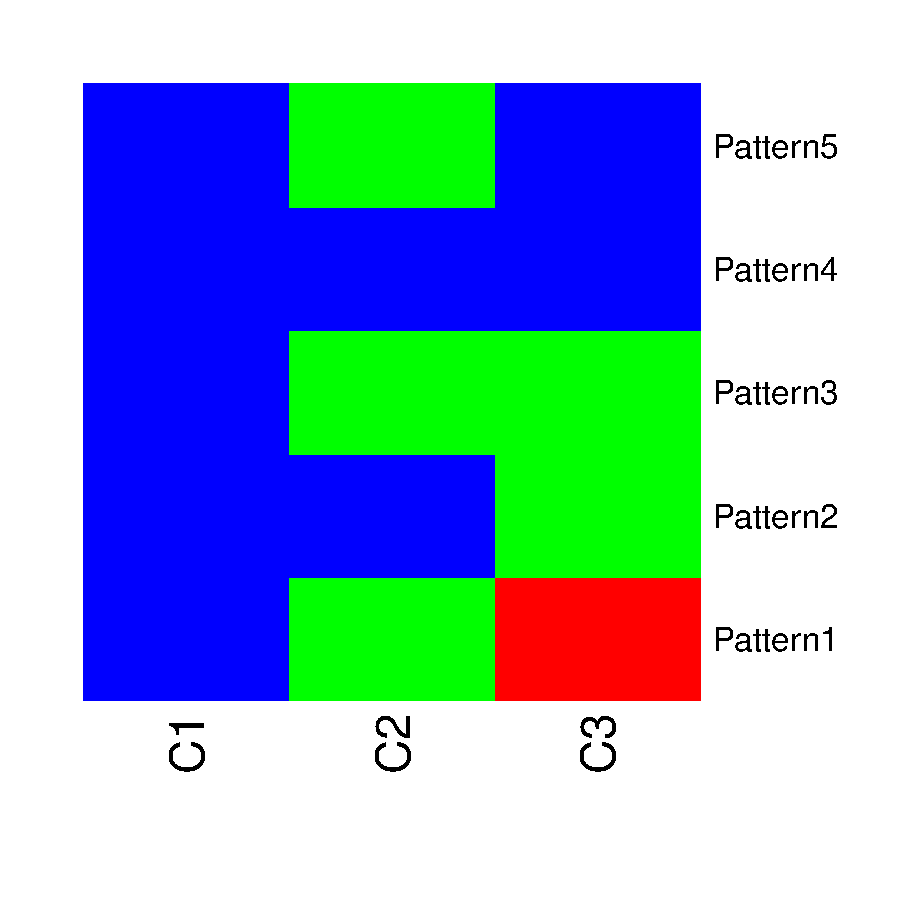
\includegraphics{EBSeq_Vignette-038}
\caption{ Selected patterns, for this case, happens to be all possible patterns for 3 conditions}
\label{fig:Patterns}
\end{figure}
\newpage
\noindent where \verb+MultiPP$PP+ provides the posterior probability of being in each pattern for every gene. 
\verb+MultiPP$MAP+ provides the most likely pattern of each gene based on the posterior 
probabilities. \verb+MultiPP$Patterns+ provides the details of the patterns.  The FC and posterior FC for multiple condition data can
be obtained by the function \verb+GetMultiFC+:

\begin{Schunk}
\begin{Sinput}
> MultiFC=GetMultiFC(MultiOut)
> str(MultiFC)
\end{Sinput}
\begin{Soutput}
List of 6
 $ FCMat         : num [1:500, 1:3] 1.217 0.951 1.069 0.923 0.983 ...
  ..- attr(*, "dimnames")=List of 2
  .. ..$ : chr [1:500] "Gene_1" "Gene_3" "Gene_5" "Gene_7" ...
  .. ..$ : chr [1:3] "C1 Over C2" "C1 Over C3" "C2 Over C3"
 $ Log2FCMat     : num [1:500, 1:3] 0.2828 -0.0724 0.0969 -0.1151 -0.0251 ...
  ..- attr(*, "dimnames")=List of 2
  .. ..$ : chr [1:500] "Gene_1" "Gene_3" "Gene_5" "Gene_7" ...
  .. ..$ : chr [1:3] "C1 Over C2" "C1 Over C3" "C2 Over C3"
 $ PostFCMat     : num [1:500, 1:3] 1.216 0.951 1.069 0.923 0.983 ...
  ..- attr(*, "dimnames")=List of 2
  .. ..$ : chr [1:500] "Gene_1" "Gene_3" "Gene_5" "Gene_7" ...
  .. ..$ : chr [1:3] "C1 Over C2" "C1 Over C3" "C2 Over C3"
 $ Log2PostFCMat : num [1:500, 1:3] 0.2822 -0.0722 0.0967 -0.115 -0.0251 ...
  ..- attr(*, "dimnames")=List of 2
  .. ..$ : chr [1:500] "Gene_1" "Gene_3" "Gene_5" "Gene_7" ...
  .. ..$ : chr [1:3] "C1 Over C2" "C1 Over C3" "C2 Over C3"
 $ CondMeans     : num [1:500, 1:3] 499 253 813 1843 753 ...
  ..- attr(*, "dimnames")=List of 2
  .. ..$ : NULL
  .. ..$ : chr [1:3] "C1" "C2" "C3"
 $ ConditionOrder: Factor w/ 3 levels "C1","C2","C3": 1 1 2 2 3 3
\end{Soutput}
\end{Schunk}

\noindent To generate a QQ-plot of the fitted Beta prior distribution 
and the $\hat{q}^C$'s within condition, a user could also use function 
\verb+DenNHist+ and \verb+QQP+.

\begin{figure}[h!]
\centering
\begin{Schunk}
\begin{Sinput}
> par(mfrow=c(2,2))
> QQP(MultiOut)
\end{Sinput}
\end{Schunk}
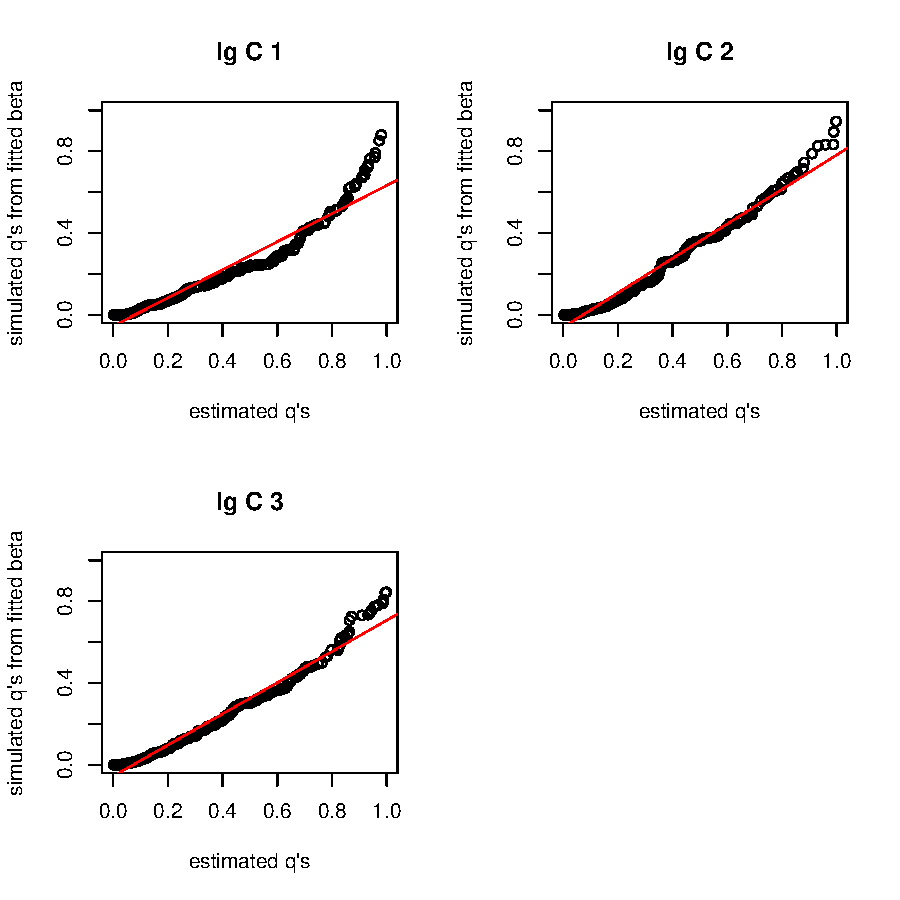
\includegraphics{EBSeq_Vignette-040}
\caption{ QQ-plots of the fitted prior distributions within each condition and each Ig group}
\label{fig:GeneMultiQQ}
\end{figure}

\begin{figure}[h]
\centering
\begin{Schunk}
\begin{Sinput}
> par(mfrow=c(2,2))
> DenNHist(MultiOut)
\end{Sinput}
\end{Schunk}
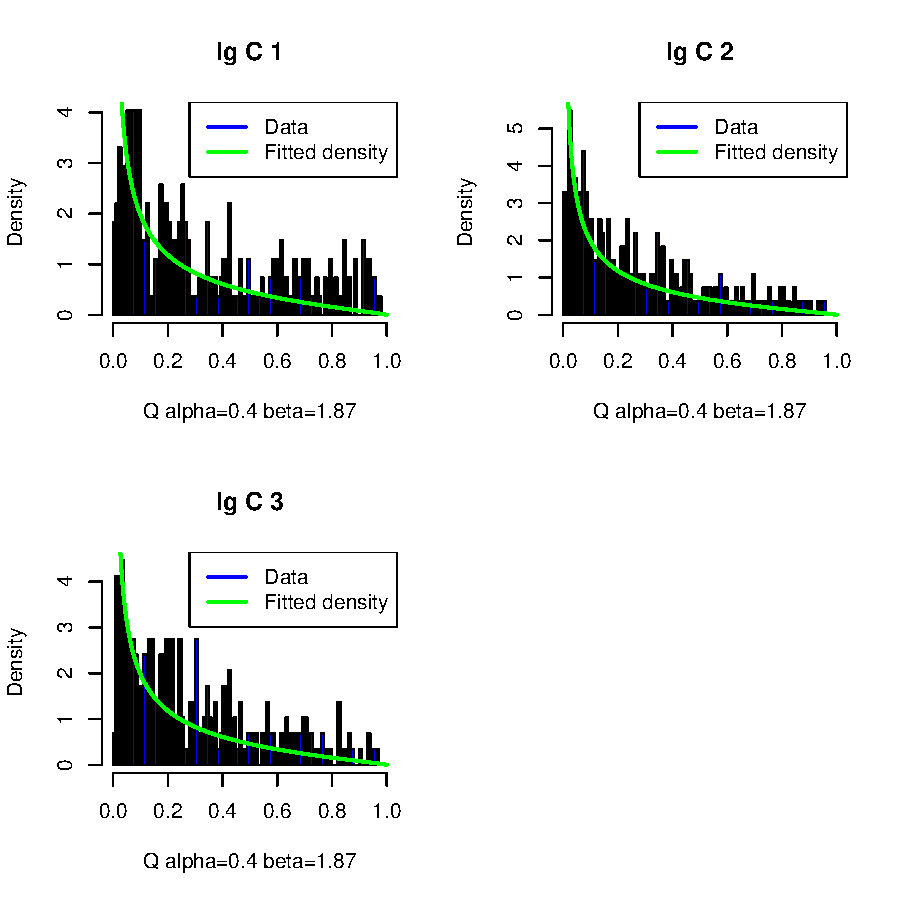
\includegraphics{EBSeq_Vignette-041}
\caption{ Prior distributions fit within each condition. 
(Note only a small set of genes are considered here for demonstration.
Better fitting should be expected while using full set of genes.)}
\label{fig:GeneMultiDenNHist}
\end{figure}
\newpage
\clearpage
\newpage
\subsection{Isoform level DE analysis (more than two conditions)}
\label{sec:detailedisomulticond}

\begin{Schunk}
\begin{Sinput}
> data(IsoMultiList)
> Conditions=c("C1","C1","C2","C2","C3","C3","C4","C4")
> IsoMultiMat=IsoMultiList[[1]]
> IsoNames.Multi=IsoMultiList$IsoNames
> IsosGeneNames.Multi=IsoMultiList$IsosGeneNames
> IsoMultiSize=MedianNorm(IsoMultiMat)
> NgList.Multi=GetNg(IsoNames.Multi, IsosGeneNames.Multi)
> IsoNgTrun.Multi=NgList.Multi$IsoformNgTrun
> IsoMultiOut=EBMultiTest(IsoMultiMat,NgVector=IsoNgTrun.Multi,Conditions=Conditions,
+ sizeFactors=IsoMultiSize, uc = 2)
> IsoMultiPP=GetMultiPP(IsoMultiOut)
\end{Sinput}
\end{Schunk}
\begin{Schunk}
\begin{Sinput}
> names(MultiPP)
\end{Sinput}
\begin{Soutput}
[1] "PP"       "MAP"      "Patterns"
\end{Soutput}
\begin{Sinput}
> IsoMultiPP$PP[1:10,]
\end{Sinput}
\begin{Soutput}
             pattern1     pattern2     pattern3     pattern4     pattern5
Iso_1_1  9.944829e-01 2.487951e-03 1.268388e-03 1.758950e-03 1.771681e-06
Iso_1_2  9.912427e-01 2.969262e-03 3.149008e-03 2.634129e-03 4.875175e-06
Iso_1_3  9.511978e-01 3.810283e-02 8.491698e-03 2.162905e-03 4.476499e-05
Iso_1_4  9.894764e-01 5.116263e-03 2.454048e-03 2.946992e-03 6.317775e-06
Iso_1_5  9.991552e-01 7.293563e-05 1.735210e-04 5.983095e-04 2.165350e-08
Iso_1_6  5.281437e-05 9.992943e-01 7.313762e-07 3.257042e-05 6.196223e-04
Iso_1_7  9.934368e-01 1.784738e-03 2.173345e-03 2.602521e-03 2.640945e-06
Iso_1_8  8.288801e-01 1.595626e-01 1.813693e-03 9.599158e-03 1.444232e-04
Iso_1_9  7.704437e-01 2.182868e-01 2.149635e-03 8.906145e-03 2.136948e-04
Iso_1_10 9.913102e-01 3.714386e-03 2.129945e-03 2.838316e-03 4.514167e-06
              pattern6      pattern7      pattern8      pattern9     pattern10
Iso_1_1   6.547737e-32  7.334070e-28  7.444297e-33  1.187580e-33  7.826127e-30
Iso_1_2   6.429034e-14  2.381428e-15  3.864389e-16  1.449241e-15  4.027626e-15
Iso_1_3   1.182199e-46  6.734763e-38  9.816011e-42  1.000115e-47  9.124439e-46
Iso_1_4   6.216584e-35  1.237632e-20  2.301442e-30  6.596860e-32  7.318319e-23
Iso_1_5   0.000000e+00  0.000000e+00  0.000000e+00  0.000000e+00  0.000000e+00
Iso_1_6  4.033350e-234 4.955181e-156 1.142613e-221 3.682627e-183 3.684941e-101
Iso_1_7  5.630249e-138 6.431489e-104 1.006944e-132 2.204727e-135 3.261238e-110
Iso_1_8  1.467526e-138  2.610835e-67 3.869222e-105 8.031404e-123  4.969433e-88
Iso_1_9   3.352994e-47  2.274798e-45  1.364332e-50  1.007720e-43  8.001378e-30
Iso_1_10  5.983367e-08  1.870470e-06  1.057221e-09  1.094014e-09  6.574554e-07
             pattern11     pattern12
Iso_1_1   4.409921e-34  4.382372e-30
Iso_1_2   1.304877e-17  2.614705e-17
Iso_1_3   8.498244e-50  8.269050e-39
Iso_1_4   5.692183e-33  1.574014e-22
Iso_1_5   0.000000e+00  0.000000e+00
Iso_1_6  2.865219e-189 5.592363e-154
Iso_1_7  2.057379e-128 3.871764e-106
Iso_1_8  5.645298e-120  2.330319e-68
Iso_1_9   4.875946e-46  3.238016e-46
Iso_1_10  1.013843e-09  1.764817e-08
\end{Soutput}
\begin{Sinput}
> IsoMultiPP$MAP[1:10]
\end{Sinput}
\begin{Soutput}
   Iso_1_1    Iso_1_2    Iso_1_3    Iso_1_4    Iso_1_5    Iso_1_6    Iso_1_7 
"pattern1" "pattern1" "pattern1" "pattern1" "pattern1" "pattern2" "pattern1" 
   Iso_1_8    Iso_1_9   Iso_1_10 
"pattern1" "pattern1" "pattern1" 
\end{Soutput}
\begin{Sinput}
> IsoMultiPP$Patterns
\end{Sinput}
\begin{Soutput}
          C1 C2 C3 C4
Pattern1   1  1  1  2
Pattern2   1  1  2  3
Pattern3   1  2  2  3
Pattern4   1  2  1  3
Pattern5   1  2  3  4
Pattern6   1  1  1  1
Pattern7   1  2  1  2
Pattern8   1  1  2  1
Pattern9   1  2  1  1
Pattern10  1  1  2  2
Pattern11  1  2  2  2
Pattern12  1  2  3  2
\end{Soutput}
\begin{Sinput}
> IsoMultiFC=GetMultiFC(IsoMultiOut)
\end{Sinput}
\end{Schunk}

Similar to Section \ref{sec:startmulticond}, 
the function \verb+GetPatterns+ allows a user to get selected patterns.
To visualize the patterns, the function \verb+PlotPattern+ may be used.
\begin{Schunk}
\begin{Sinput}
> PosParti.4Cond=GetPatterns(IsoMultiOut)
> PosParti.4Cond
\end{Sinput}
\begin{Soutput}
          C1 C2 C3 C4
Pattern1   1  1  1  2
Pattern2   1  1  2  3
Pattern3   1  2  2  3
Pattern4   1  2  1  3
Pattern5   1  2  3  4
Pattern6   1  1  1  1
Pattern7   1  2  1  2
Pattern8   1  1  2  1
Pattern9   1  2  1  1
Pattern10  1  1  2  2
Pattern11  1  2  2  2
Pattern12  1  2  3  2
\end{Soutput}
\end{Schunk}

\begin{figure}[h!]
\centering
\begin{Schunk}
\begin{Sinput}
> PlotPattern(PosParti.4Cond)
\end{Sinput}
\end{Schunk}
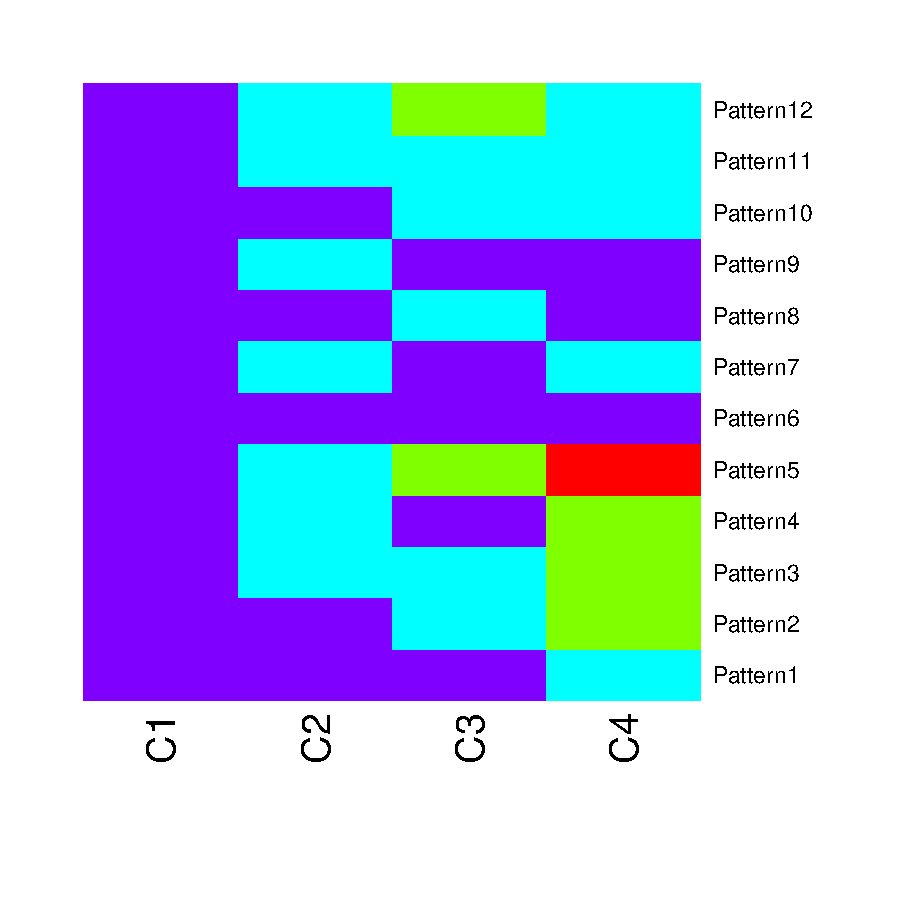
\includegraphics{EBSeq_Vignette-045}
\caption{Selected patterns for 4 conditions}
\label{fig:Patterns4Cond}
\end{figure}
\newpage


The FC and posterior FC for multiple condition data can be obtained by the function \verb+GetMultiFC+:


\noindent To generate a QQ-plot of the fitted Beta prior distribution 
and the $\hat{q}^C$'s within condition, a user could also use the functions 
\verb+DenNHist+ and \verb+QQP+.
\newpage
\begin{figure}[h!]
\centering
\begin{Schunk}
\begin{Sinput}
> par(mfrow=c(3,4))
> QQP(IsoMultiOut)
> 
\end{Sinput}
\end{Schunk}
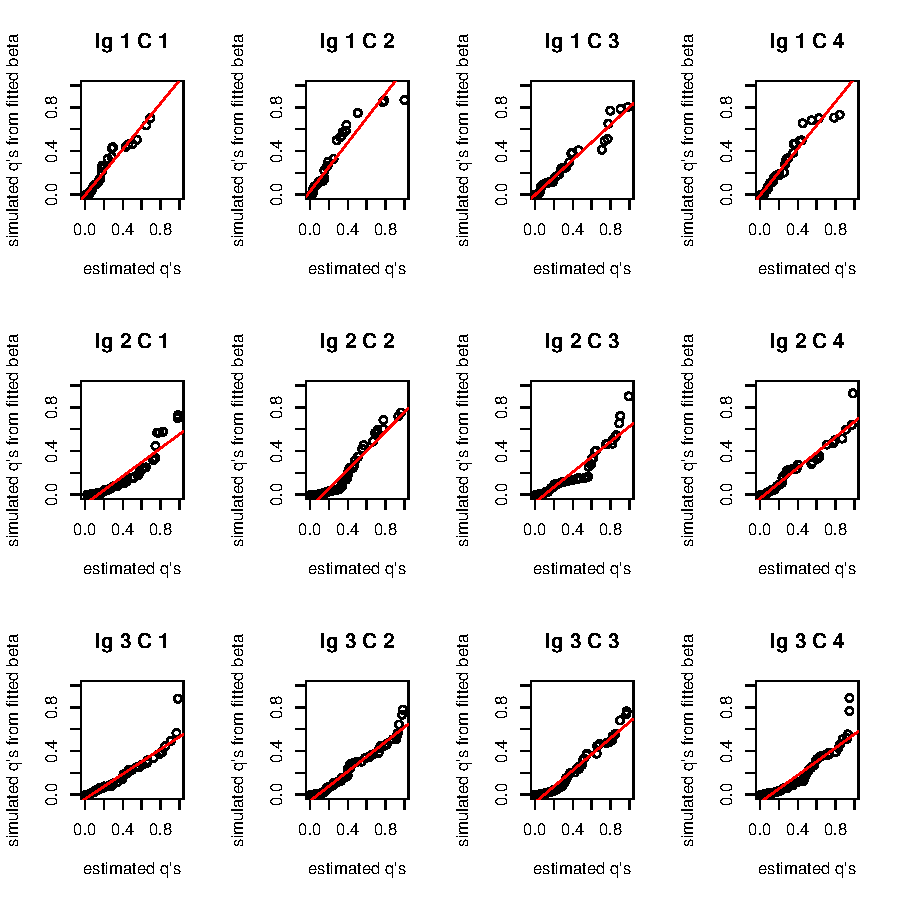
\includegraphics{EBSeq_Vignette-046}
\caption{ QQ-plots of the fitted prior distributions within each condition and Ig group. 
(Note only a small set of isoforms are considered here for demonstration.
Better fitting should be expected while using full set of isoforms.)}
\label{fig:IsoMultiQQ}
\end{figure}

\begin{figure}[h]
\centering
\begin{Schunk}
\begin{Sinput}
> par(mfrow=c(3,4))
> DenNHist(IsoMultiOut)
\end{Sinput}
\end{Schunk}
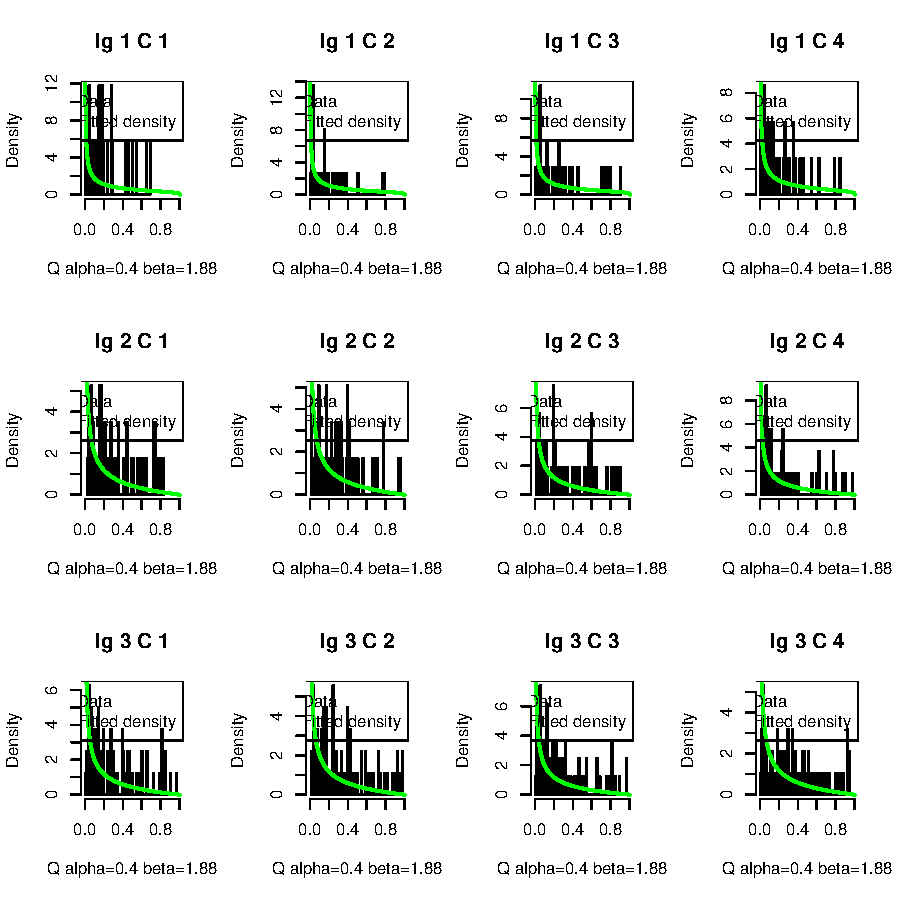
\includegraphics{EBSeq_Vignette-047}
\caption{ Prior distributions fit within each condition and Ig group. 
(Note only a small set of isoforms are considered here for demonstration.
Better fitting should be expected while using full set of isoforms.)}
\label{fig:IsoMultiDenNHist}
\end{figure}
\clearpage
\newpage


\newpage
\subsection{Working without replicates}
When replicates are not available, it is difficult to estimate the transcript specific variance.
In this case, EBSeq estimates the variance by  pooling similar genes together.  
Specifically, we take genes with FC in the 25\% - 75\% quantile of all FC's as 
candidate genes. By defining \verb+NumBin = 1000+ (default in \verb+EBTest+), EBSeq 
will group genes with similar means into 1,000 bins. 
For each candidate gene, we use the across-condition variance estimate as its variance estimate. 
For each bin, the bin-wise variance estimation is taken to be the median of the 
across-condition variance estimates of the candidate genes within that bin. 
For each non-candidate gene, we use the bin-wise variance estimate of the host bin (the bin containing this gene) 
as its variance estimate.
This approach works well when there are no more than 50\% DE genes in the data set. 

\subsubsection{Gene counts with two conditions}
\label{sec:norepgenede}

To generate a data set with no replicates, we take the first sample of each condition. 
For example, using the data from Section \ref{sec:detailedgenede}, we take sample 1 from condition 1 and 
sample 6 from condition 2. Functions \verb+MedianNorm+, \verb+GetDEResults+ and 
\verb+PostFC+ may be used on data without replicates.
\begin{Schunk}
\begin{Sinput}
> data(GeneMat)
> GeneMat.norep=GeneMat[,c(1,6)]
> Sizes.norep=MedianNorm(GeneMat.norep)
> EBOut.norep=EBTest(Data=GeneMat.norep,
+ Conditions=as.factor(rep(c("C1","C2"))),
+ sizeFactors=Sizes.norep)
\end{Sinput}
\begin{Soutput}
Removing transcripts with 100 th quantile < = 0 
999 transcripts will be tested
Initial number of DE patterns = 2
Final number of DE patterns = 2
\end{Soutput}
\begin{Sinput}
> EBDERes.norep=GetDEResults(EBOut.norep)
> GeneFC.norep=PostFC(EBOut.norep)
\end{Sinput}
\end{Schunk}

\subsubsection{Isoform counts with two conditions}
\label{norepisode}
To generate an isoform level data set with no replicates, we
also take sample 1 and sample 6 in the data we used in Section
\ref{sec:detailedisode}. 
Example codes are shown below.

\begin{Schunk}
\begin{Sinput}
> data(IsoList)
> IsoMat=IsoList$IsoMat
> IsoNames=IsoList$IsoNames
> IsosGeneNames=IsoList$IsosGeneNames
> NgList=GetNg(IsoNames, IsosGeneNames)
> IsoNgTrun=NgList$IsoformNgTrun
> IsoMat.norep=IsoMat[,c(1,6)]
> IsoSizes.norep=MedianNorm(IsoMat.norep)
> IsoEBOut.norep=EBTest(Data=IsoMat.norep, NgVector=IsoNgTrun,
+ Conditions=as.factor(c("C1","C2")),
+ sizeFactors=IsoSizes.norep)
\end{Sinput}
\begin{Soutput}
Removing transcripts with 100 th quantile < = 0 
1192 transcripts will be tested
Initial number of DE patterns = 2
Final number of DE patterns = 2
\end{Soutput}
\begin{Sinput}
> IsoEBDERes.norep=GetDEResults(IsoEBOut.norep)
> IsoFC.norep=PostFC(IsoEBOut.norep)
\end{Sinput}
\end{Schunk}

\subsubsection{Gene counts with more than two conditions}
\label{norepisode}
To generate a data set with multiple conditions and no replicates, 
we take the first sample from each condition (sample 1, 3 and 5) in the data we used
in Section \ref{sec:detailedmulticond}. 
Example codes are shown below.
\begin{Schunk}
\begin{Sinput}
> data(MultiGeneMat)
> MultiGeneMat.norep=MultiGeneMat[,c(1,3,5)]
> Conditions=c("C1","C2","C3")
> #PosParti=GetPatterns(Conditions)
> #Parti=PosParti[-3,]
> MultiSize.norep=MedianNorm(MultiGeneMat.norep)
> MultiOut.norep=EBMultiTest(MultiGeneMat.norep,
+ NgVector=NULL,Conditions=Conditions, sizeFactors=MultiSize.norep, 
+ uc =2)
\end{Sinput}
\begin{Soutput}
Initial number of DE patterns = 5
Final number of DE patterns = 5
\end{Soutput}
\begin{Sinput}
> MultiPP.norep=GetMultiPP(MultiOut.norep)
> MultiFC.norep=GetMultiFC(MultiOut.norep)
\end{Sinput}
\end{Schunk}

\subsubsection{Isoform counts with more than two conditions}
\label{sec:norepmulticond}
To generate an isoform level data set with multiple conditions and no replicates,
we take the first sample from each condition (sample 1, 3, 5 and 7) in the data we used
in Section \ref{sec:detailedisomulticond}. 
Example codes are shown below.



\begin{Schunk}
\begin{Sinput}
> data(IsoMultiList)
> IsoMultiMat=IsoMultiList[[1]]
> IsoNames.Multi=IsoMultiList$IsoNames
> IsosGeneNames.Multi=IsoMultiList$IsosGeneNames
> IsoMultiMat.norep=IsoMultiMat[,c(1,3,5,7)]
> IsoMultiSize.norep=MedianNorm(IsoMultiMat.norep)
> NgList.Multi=GetNg(IsoNames.Multi, IsosGeneNames.Multi)
> IsoNgTrun.Multi=NgList.Multi$IsoformNgTrun
> Conditions=c("C1","C2","C3","C4")
> #PosParti.4Cond=GetPatterns(Conditions)
> #PosParti.4Cond
> #Parti.4Cond=PosParti.4Cond[c(1,2,3,8,15),]
> #Parti.4Cond
> IsoMultiOut.norep=EBMultiTest(IsoMultiMat.norep,
+ NgVector=IsoNgTrun.Multi,Conditions=Conditions,
+ sizeFactors=IsoMultiSize.norep, uc = 3)
\end{Sinput}
\begin{Soutput}
Initial number of DE patterns = 14
Final number of DE patterns = 14
\end{Soutput}
\begin{Sinput}
> IsoMultiPP.norep=GetMultiPP(IsoMultiOut.norep)
> IsoMultiFC.norep=GetMultiFC(IsoMultiOut.norep)
\end{Sinput}
\end{Schunk}

\section{EBSeq pipelines and extensions}
\subsection{RSEM-EBSeq pipeline: from raw reads to differential expression analysis results}
EBSeq is coupled with RSEM \cite{Li11b} as an RSEM-EBSeq pipeline which provides 
quantification and DE testing on both gene and isoform levels.

For more details, see 
\url{http://deweylab.biostat.wisc.edu/rsem/README.html#de}

\subsection{EBSeq interface: A user-friendly graphical interface for differetial expression analysis}
EBSeq interface provides a graphical interface implementation for users who are not familiar with the R 
programming language. It takes .xls, .xlsx and .csv files as input. 
Additional packages need be downloaded; they may be found at
\url{http://www.biostat.wisc.edu/~ningleng/EBSeq_Package/EBSeq_Interface/}

\subsection{EBSeq Galaxy tool shed}
EBSeq tool shed contains EBSeq wrappers for a local Galaxy implementation.
For more details, see
\url{http://www.biostat.wisc.edu/~ningleng/EBSeq_Package/EBSeq_Galaxy_toolshed/}

\section{Acknowledgment}
We would like to thank Haolin Xu for checking the package and
proofreading the vignette.

\section{News}
2014-1-30: In EBSeq 1.3.3, the default setting of EBTest function will remove
low expressed genes (genes whose 75th quantile of normalized counts is less
than 10) before identifying DE genes.
These two thresholds can be changed in EBTest function.
Because low expressed genes are disproportionately noisy, 
removing these genes prior to downstream analyses can improve model fitting and increase robustness
(e.g. by removing outliers).

2014-5-22: In EBSeq 1.5.2, numerical approximations are implemented to deal with
underflow. The underflow is likely due to large number of samples.

2015-1-29: In EBSeq 1.7.1, EBSeq incorporates a new function
GetDEResults() which may be used to obtain a list of transcripts under a target FDR in a two-condition experiment.
The results obtained by applying this function with its default setting will be
more robust to transcripts with low variance and potential outliers.
By using the default settings in this function,
the number of genes identified in any given analysis may
differ slightly from the previous version (1.7.0 or order). 
To obtain results that are comparable
to results from earlier versions of EBSeq (1.7.0 or older), a user may set
Method="classic" in GetDEResults() function, or use the original GetPPMat() function.
The GeneDEResults() function also allows a user to modify thresholds to
target genes/isoforms with a pre-specified posterior fold change.

Also, in EBSeq 1.7.1, the default settings in EBTest() and EBMultiTest() function
will only remove transcripts with all 0's (instead of removing transcripts with 
75th quantile less than 10 in version 1.3.3-1.7.0).
To obtain a list of transcripts comparable to the results generated by     EBSeq version 1.3.3-1.7.0, a user may change Qtrm = 0.75 and QtrmCut = 10
when applying EBTest() or EBMultiTest() function.

\section{Common Q and A}
\subsection{Read in data}

csv file:

\verb+In=read.csv("FileName", stringsAsFactors=F, row.names=1, header=T)+

\verb+Data=data.matrix(In)+

\noindent txt file:

\verb+In=read.table("FileName", stringsAsFactors=F, row.names=1, header=T)+

\verb+Data=data.matrix(In)+

\noindent Check \verb+str(Data)+ and make sure it is a matrix instead of data frame. You may need to play around with the \verb+row.names+ 
and \verb+header+ option depends on how the input file was generated.



\subsection{GetDEResults() function not found}

You may on an earlier version of EBSeq. The GetDEResults function
was introduced since version 1.7.1.
The latest release version could be found at:

\url{http://www.bioconductor.org/packages/release/bioc/html/EBSeq.html}

\noindent The latest devel version:

\url{http://www.bioconductor.org/packages/devel/bioc/html/EBSeq.html}

\noindent And you may check your package version by typing \verb+packageVersion("EBSeq")+.


\subsection{Visualizing DE genes/isoforms}

To generate a heatmap, you may consider the heatmap.2 function in gplots package.
For example, you may run

\verb+heatmap.2(NormalizedMatrix[GenesOfInterest,], scale="row", trace="none", Colv=F)+

The normalized matrix may be obtained from \verb+GetNormalizedMat()+ function.


\subsection{My favorite gene/isoform has NA in PP (status "NoTest")}

\indent The NoTest status comes from two sources:

1) In version 1.3.3-1.7.0, using the default parameter settings of EBMultiTest(), the function
will not test on genes with more than 75\% values $\le$ 10 to ensure better
model fitting. To disable this filter, you may set Qtrm=1 and
QtrmCut=0.

2) numerical over/underflow in R. That happens when the within
condition variance is extremely large or small. we did implemented a numerical
approximation step to calculate the approximated PP for these genes
with over/underflow. Here we use $10^{-10}$ to approximate the parameter p
in the NB distribution for these genes (we set it to a small value
since we want to cover more over/underflow genes with low
within-condition variation). You may try to tune this value (to a larger value) in the
approximation by setting \verb+ApproxVal+ in \verb+EBTest()+ or \verb+EBMultiTest()+ function. 

\pagebreak
\bibliographystyle{plain}
\bibliography{lengetal}

\end{document}

